\documentclass{article}
\usepackage{graphicx, xcolor}
\usepackage{subcaption}
\usepackage{amsmath}
\usepackage{hyperref}
\usepackage{listings}
\usepackage{caption}
\usepackage{float}
\usepackage[margin=2.5cm]{geometry}

\title{Praktické paralelní programování\\Dokumentace k projektu č. 1\\MPI a paralelní I/O}
\author{Dominik Huml (xhumld00)}
\date{\today}

\begin{document}

\maketitle

% =========================================================
\section{Úvod}
\label{sec:uvod}
% =========================================================

Projekt implementuje paralelní simulaci šíření tepla 2D doménou pomocí
metody konečných diferencí (FDTD).
Paralelizace je realizována kombinací MPI (rozdělení domény mezi procesy)
a OpenMP (vlákna uvnitř procesu) se dvěma typy halo výměny:
komunikace bod-bod (P2P) a vzdálený přístup k paměti (RMA).
Simulace ukládá průběh do souboru HDF5 s podporou paralelního I/O.

% =========================================================
\section{Popis implementace}
\label{sec:implementace}
% =========================================================

\textbf{Dekompozice domény.}
Implementace podporuje 1D dekompozici (vodorovné pásy, $n_x = P$, $n_y = 1$)
a 2D dekompozici (čtvercové nebo obdélníkové dlaždice).
Topologie procesů je kartézská (\texttt{MPI\_Cart\_create});
sousední procesy jsou určeni pomocí \texttt{MPI\_Cart\_shift}.

\textbf{Překrytí výpočtu a komunikace.}
Každá iterace postupuje takto:
(1)~\texttt{computeHaloZones} – výpočet okrajových buněk (data k odeslání),
(2)~\texttt{startHaloExchange*} – zahájení neblokující výměny okrajů,
(3)~\texttt{updateTile} – výpočet vnitřku dlaždice za běhu komunikace,
(4)~\texttt{awaitHaloExchange*} – čekání na dokončení výměny.
Tím je komunikace skryta za výpočet vnitřku dlaždice.

\textbf{RMA synchronizace.}
Namísto globální bariéry \texttt{MPI\_Win\_fence} je použit protokol PSCW
(\texttt{MPI\_Win\_post/start/complete/wait}), který synchronizuje pouze
přímé sousedy. Na jednom uzlu zrychlení 1{,}15$\times$, na dvou uzlech
1{,}74$\times$; při škálování na 4–8 uzlů přínos dále roste.
Halo data jsou před RMA přenosem pakována pomocí \texttt{MPI\_Pack/Unpack}
do souvislého bufferu, čímž se eliminují strided přístupy.

\textbf{Paralelní I/O.}
Klíčová optimalizace: \texttt{H5Pset\_chunk} nastavena na velikost celé
globální domény místo lokální dlaždice.
S tile-sized chunks vzniká velké množství malých objektů, reálný zápis
128 procesů trval 2954\,s.
Po opravě na jeden chunk = celá doména a nastavení Lustre stripingu
(\texttt{lfs setstripe -S 1M -c 16}) klesl čas na 0{,}7\,s (\textbf{4220$\times$}).

% =========================================================
\section{Škálování}
\label{sec:skalovani}
% =========================================================

Silné škálování je měřeno na mřížkách 256–4096, 1–32 procesů (MPI 2D)
resp. 1–32 procesů $\times$ 8 vláken (Hybrid 2D) nebo 1–16 procesů
$\times$ 16 vláken (Hybrid 1D), vždy 8 uzlů Barbory, 256 jader celkem.
Referenční čas je sekvenční implementace na dané velikosti domény.

Nejlepší naměřené zrychlení je \textbf{671$\times$} pro Hybrid 2D, mřížka
4096$^2$, 256 jader, bez I/O – \emph{superlineární} oproti ideálnímu 256$\times$.
Důvod: sekvenční solver je limitován RAM (pracovní sada 256\,MB),
zatímco paralelní dlaždice ($1024 \times 512$ floatů, $\approx$\,4\,MB) se vejde
do 24{,}75\,MB L3 cache na socket, takže stencil běží z cache namísto RAM.

\medskip
\textbf{Rozdíl 1D a 2D dekompozice.}
Objem halo komunikace na proces závisí na tvaru dlaždice:
\[
  V_\text{1D} = 4N, \qquad
  V_\text{2D} = \frac{8N}{\sqrt{P}}, \qquad
  \frac{V_\text{1D}}{V_\text{2D}} = \frac{\sqrt{P}}{2}.
\]
Při $P=16$ posílá 1D \textbf{2$\times$} více dat, při $P=256$
již \textbf{8$\times$} více.
Naměřený efekt: Hybrid 1D (256 jader) dosahuje 368$\times$ zrychlení
oproti 671$\times$ Hybrid 2D – přibližně 1{,}8$\times$ horší výsledek.
V testované sadě 90 konfigurací zvítězila 2D dekompozice v 56 případech.
Zátěž je vyrovnaná – všechny procesy zpracovávají stejně velké dlaždice,
komunikační matice v nástroji Cube potvrzuje rovnoměrné rozložení odeslaných bytů.

\medskip
\textbf{Vliv I/O.}
Pro 2D Hybrid, mřížka 1024$^2$, 16 procesů:
bez I/O 0{,}72\,s, sekvenční I/O 2{,}07\,s, paralelní I/O 13{,}65\,s.
Na velkých doménách s dostatečným počtem OST disků se paralelní I/O blíží
sekvenčnímu a přibližuje se hodnotě bez I/O díky opravě chunk parametru.

% ----- MPI 2D -----
\begin{figure}[H]
    \centering
    \begin{subfigure}{0.45\textwidth}
        \centering
        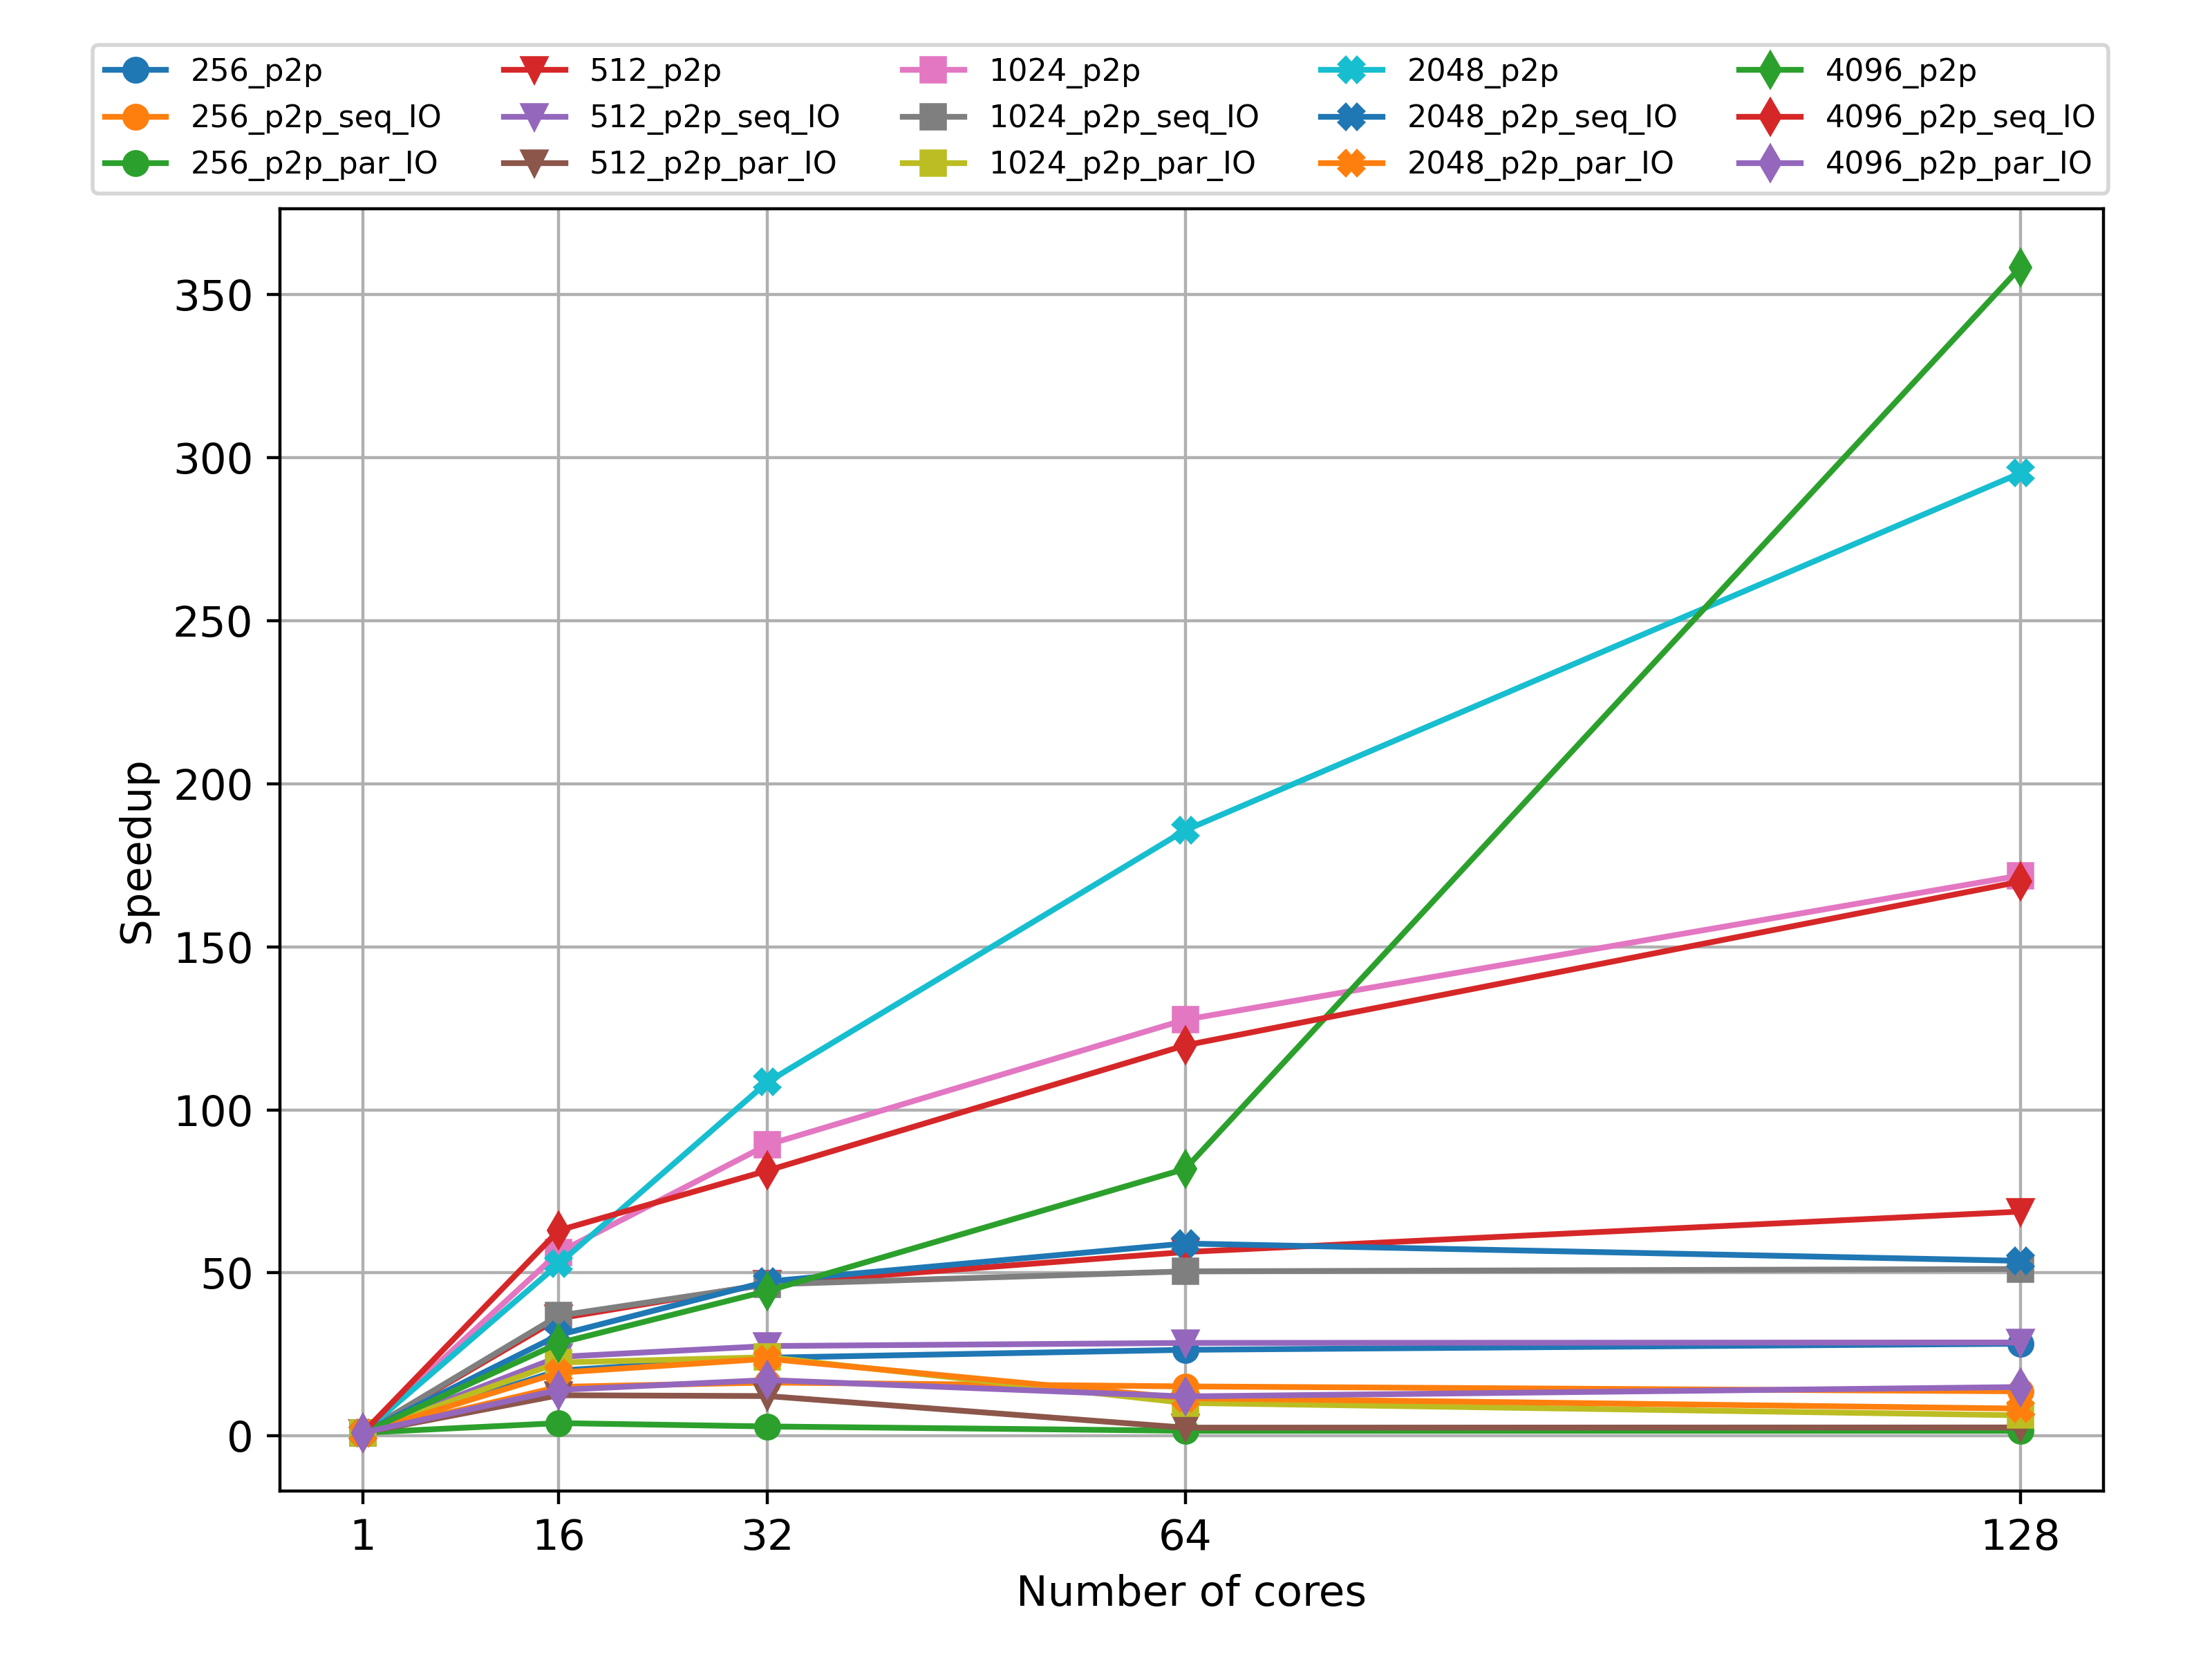
\includegraphics[width=\textwidth]{figures/ppp_speedup_mpi_p2p.png}
        \caption{Silné škálování: čisté MPI s 2D dekompozicí, P2P.}
        \label{fig:2D_MPI_P2P}
    \end{subfigure}
    \hfill
    \begin{subfigure}{0.45\textwidth}
        \centering
        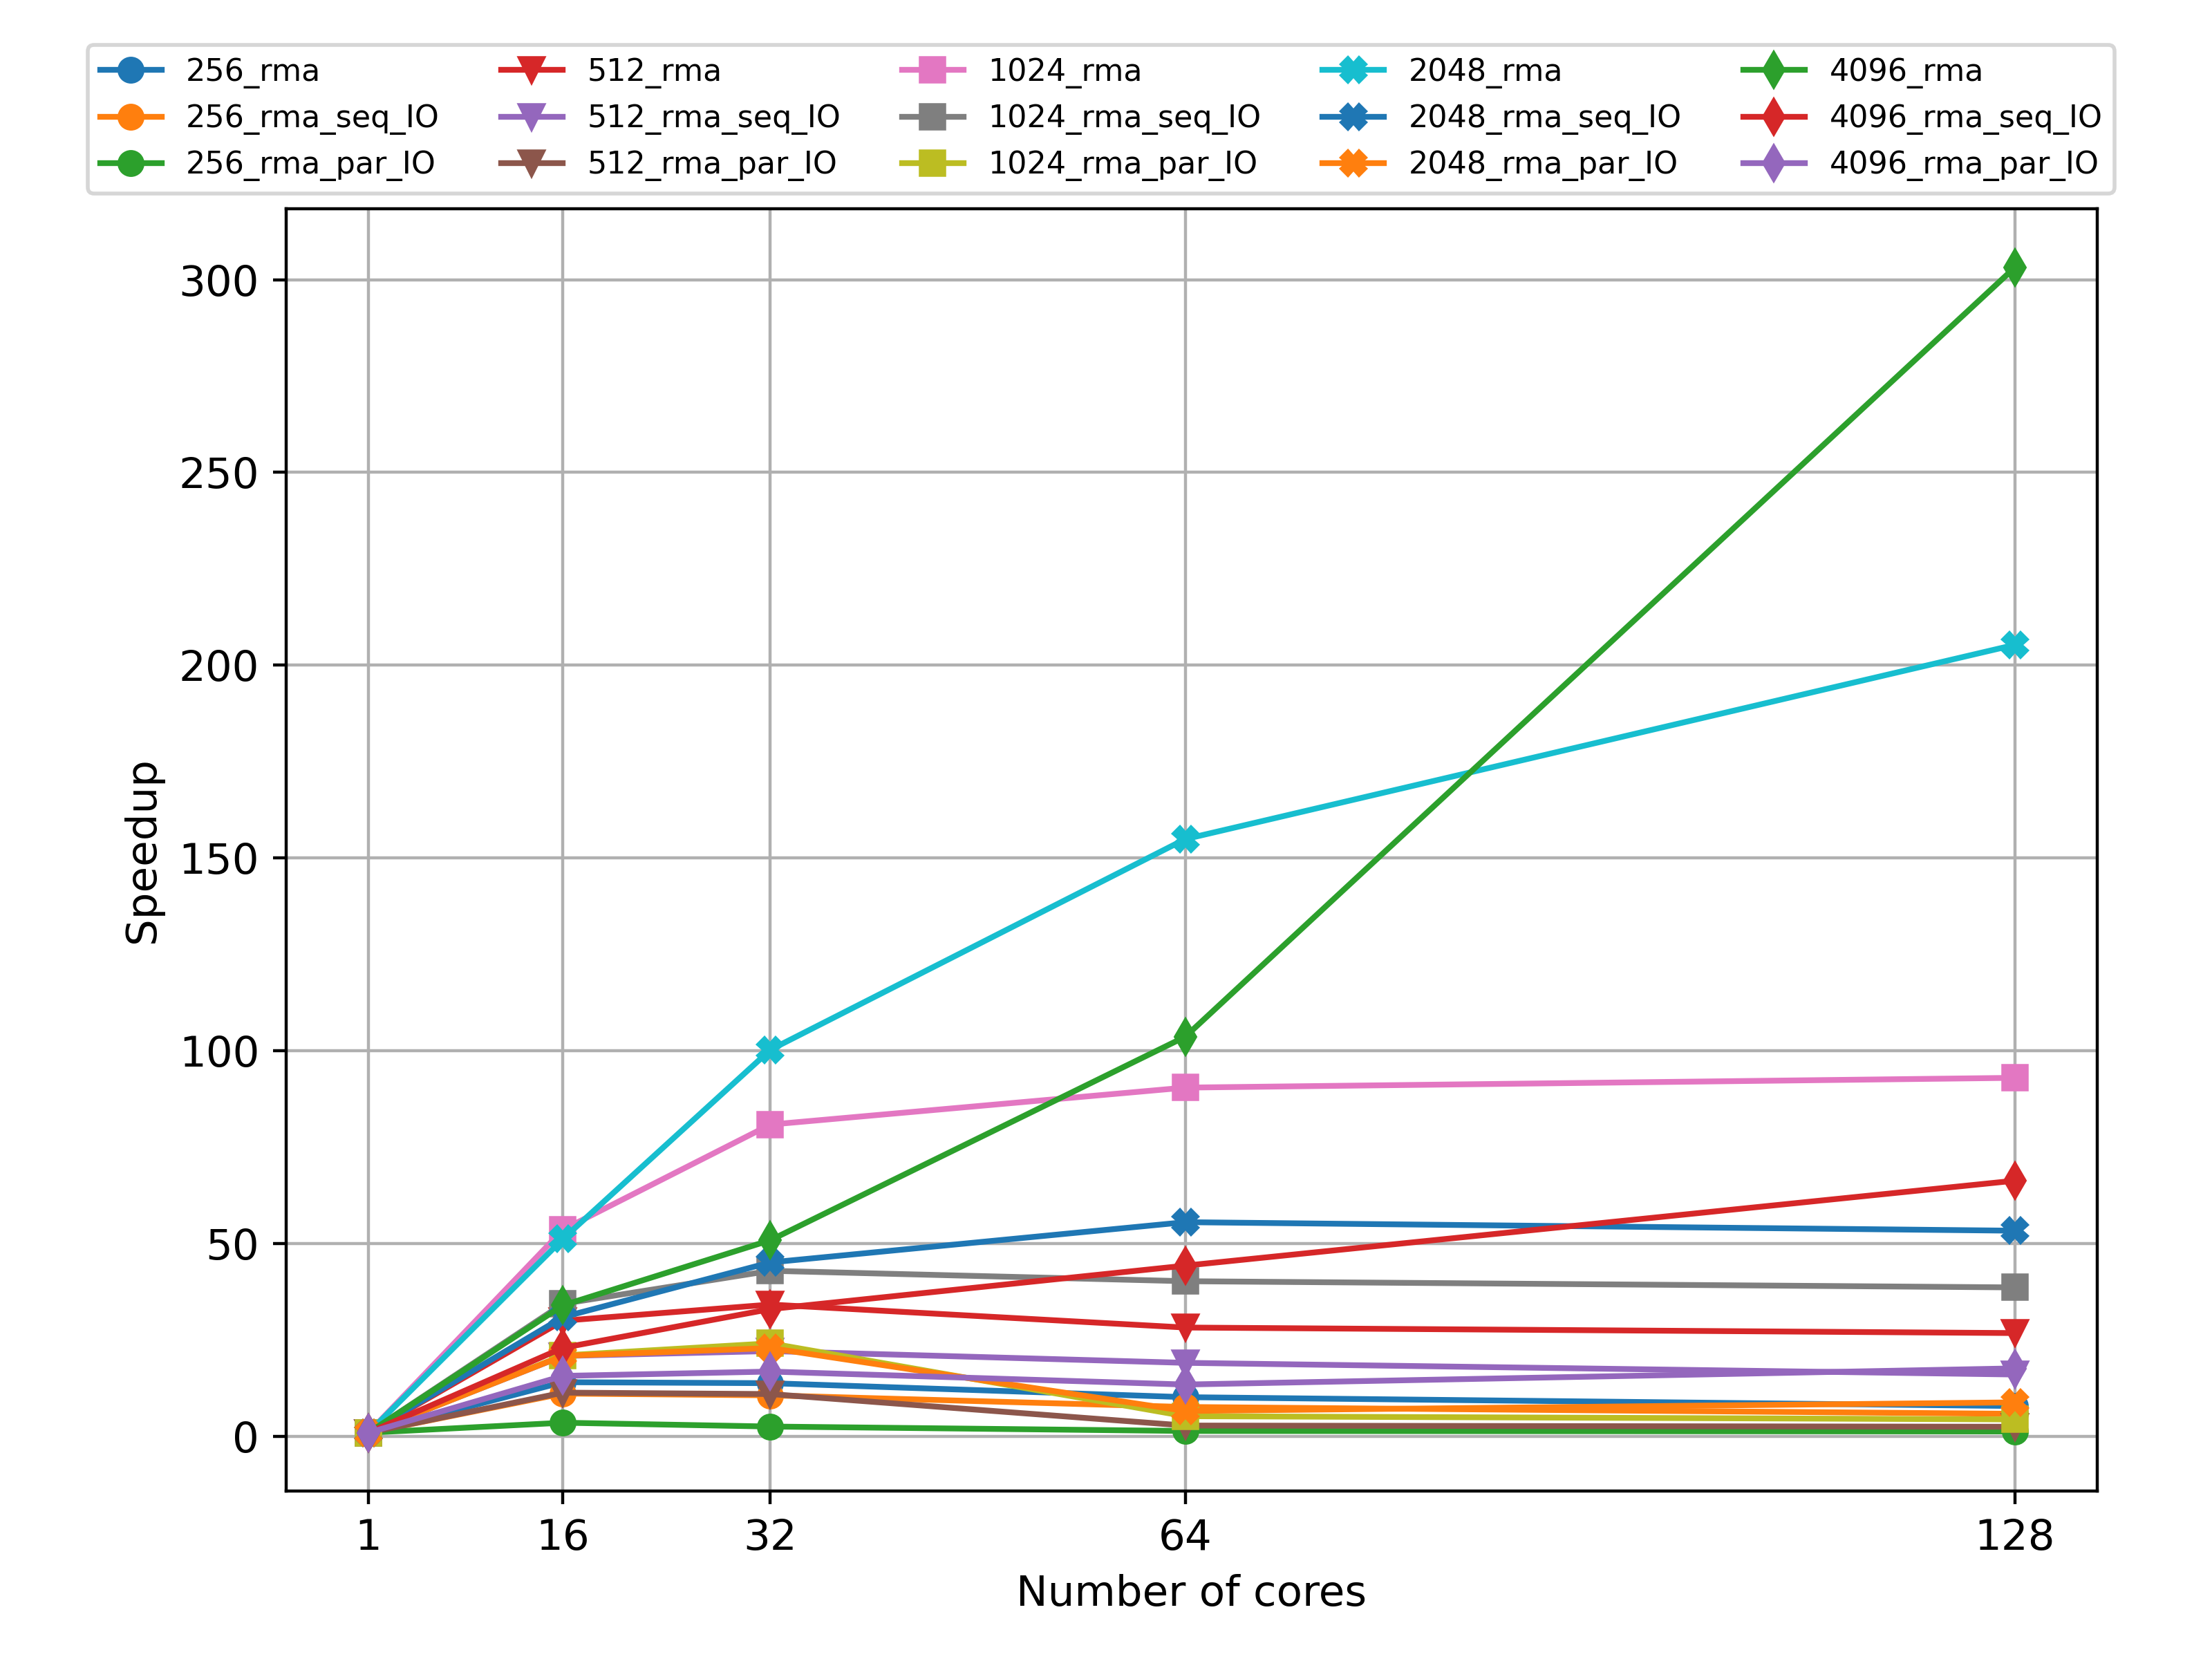
\includegraphics[width=\textwidth]{figures/ppp_speedup_mpi_rma.png}
        \caption{Silné škálování: čisté MPI s 2D dekompozicí, RMA.}
        \label{fig:2D_MPI_RMA}
    \end{subfigure}

    \begin{subfigure}{0.45\textwidth}
        \centering
        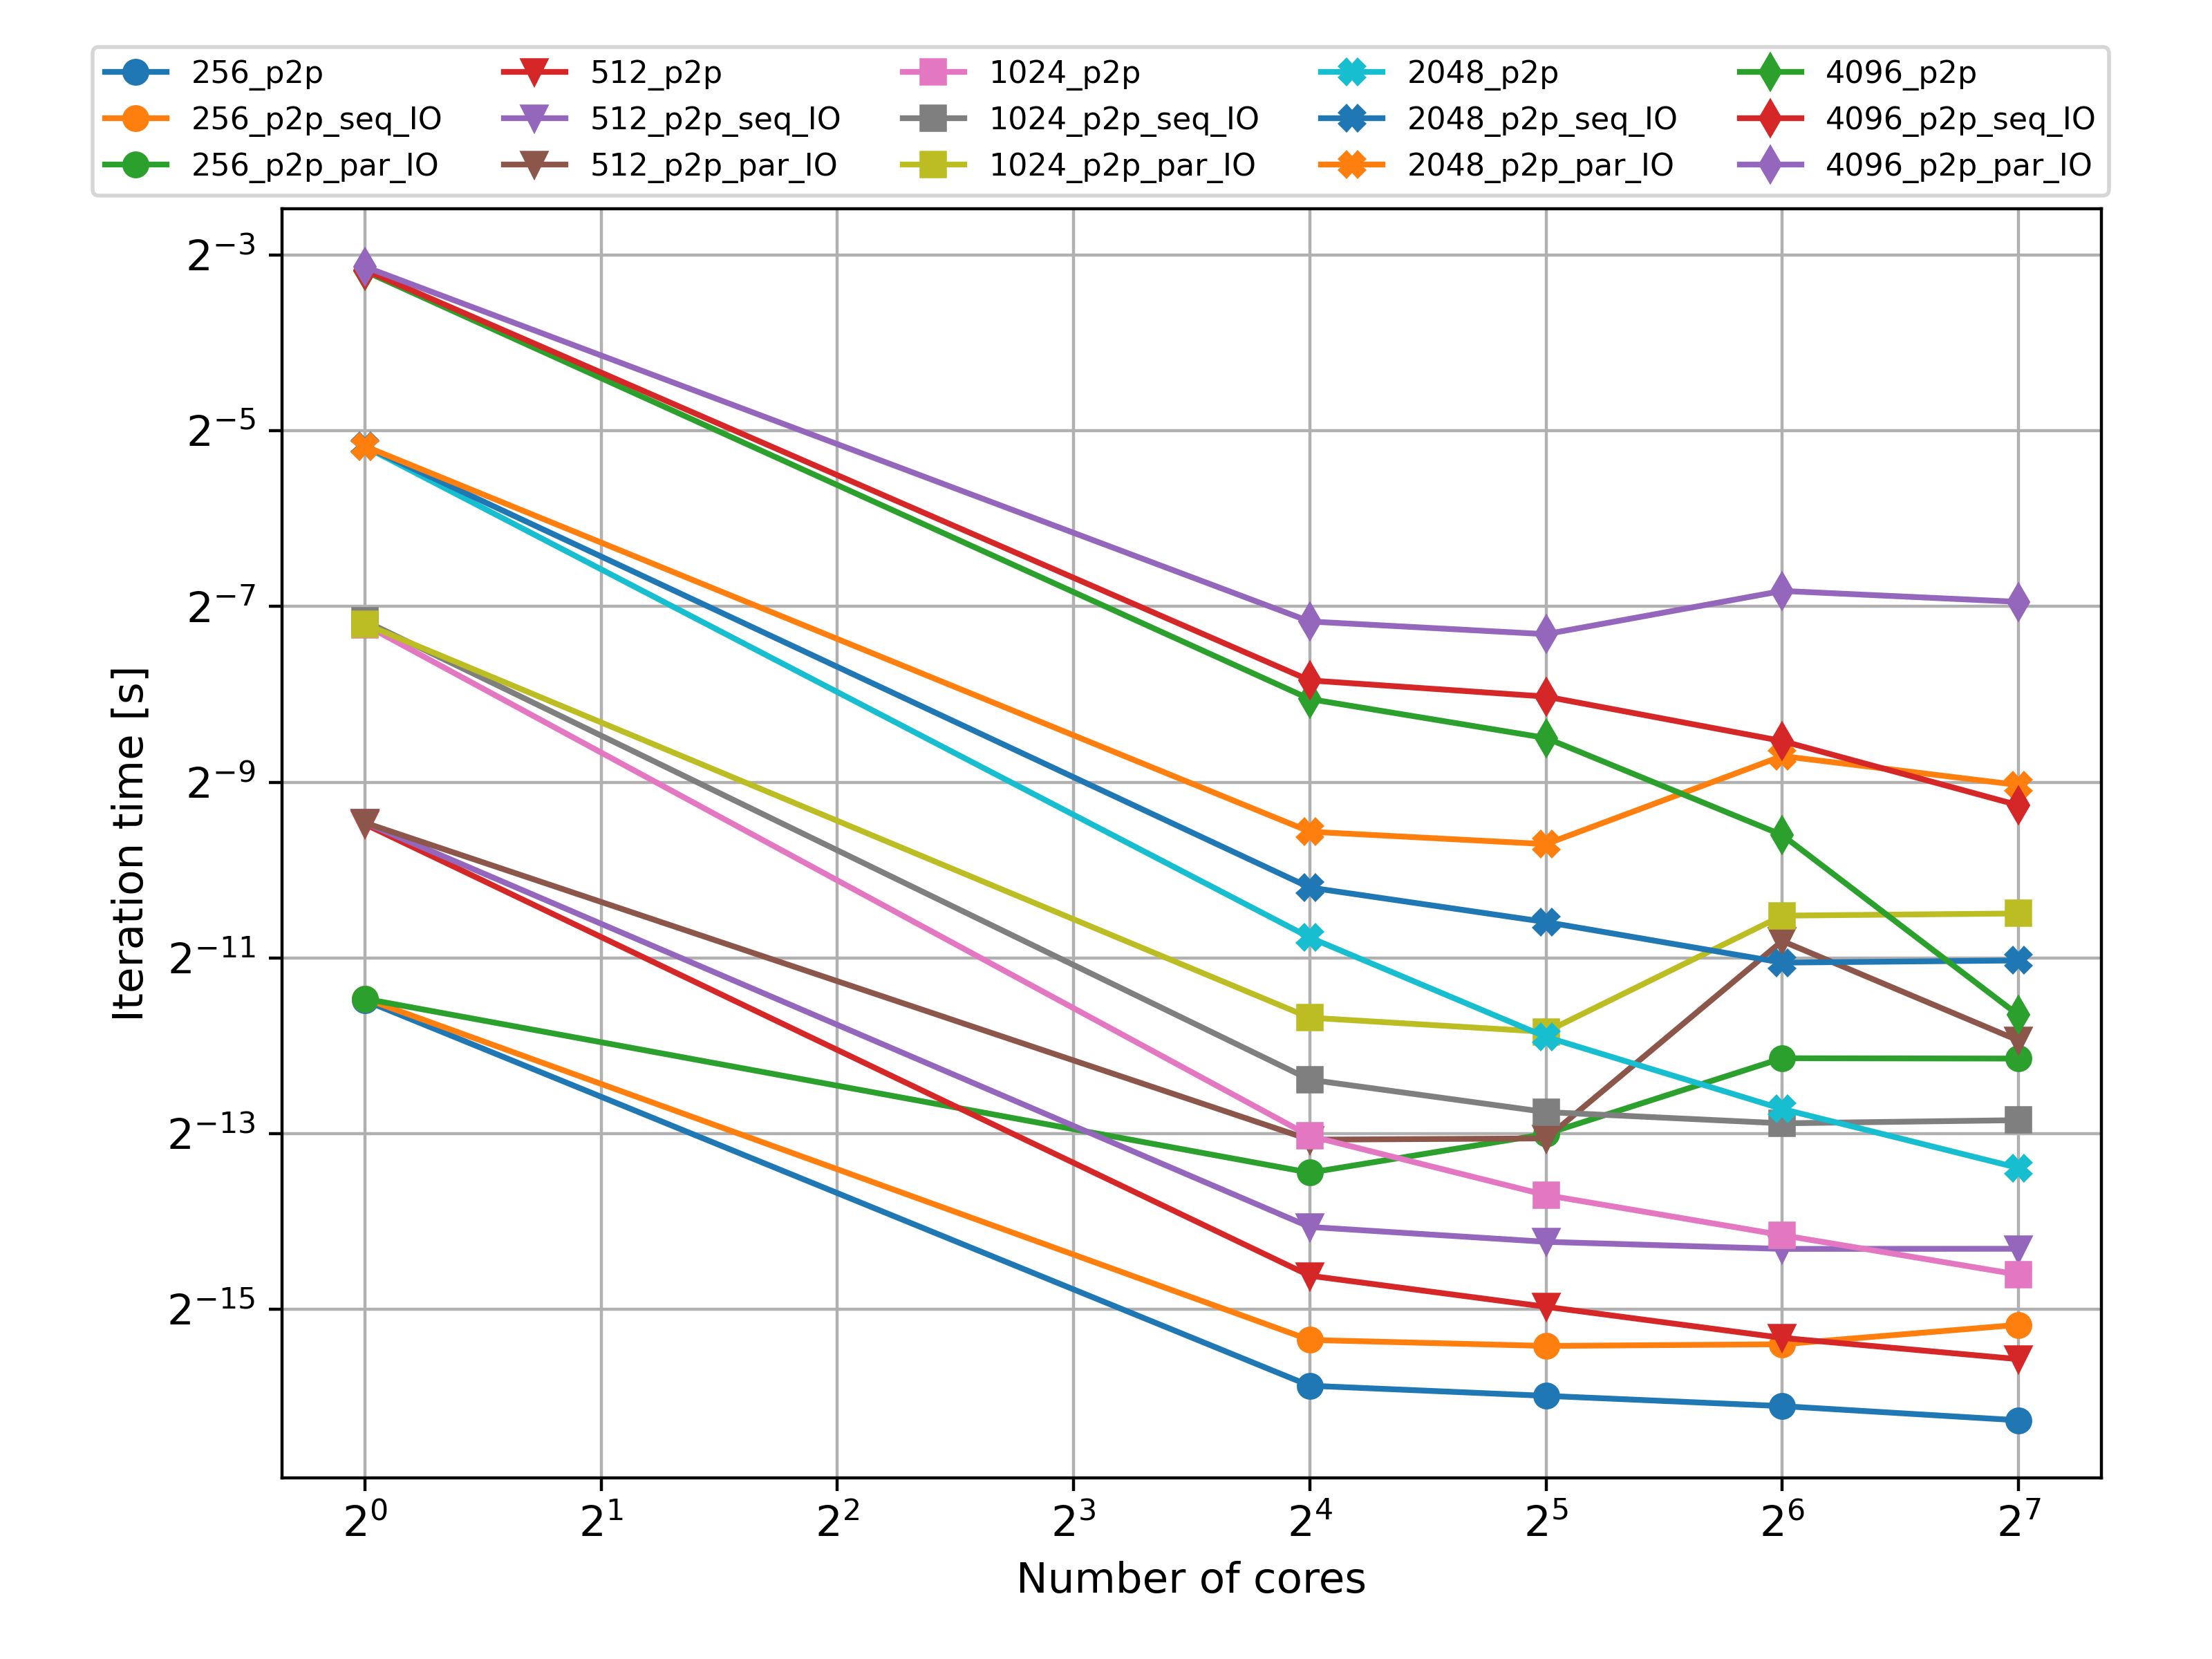
\includegraphics[width=\textwidth]{figures/ppp_scaling_mpi_p2p.png}
        \caption{Cena výpočtu: čisté MPI s 2D dekompozicí, P2P.}
        \label{fig:2D_MPI_P2P_eff}
    \end{subfigure}
    \hfill
    \begin{subfigure}{0.45\textwidth}
        \centering
        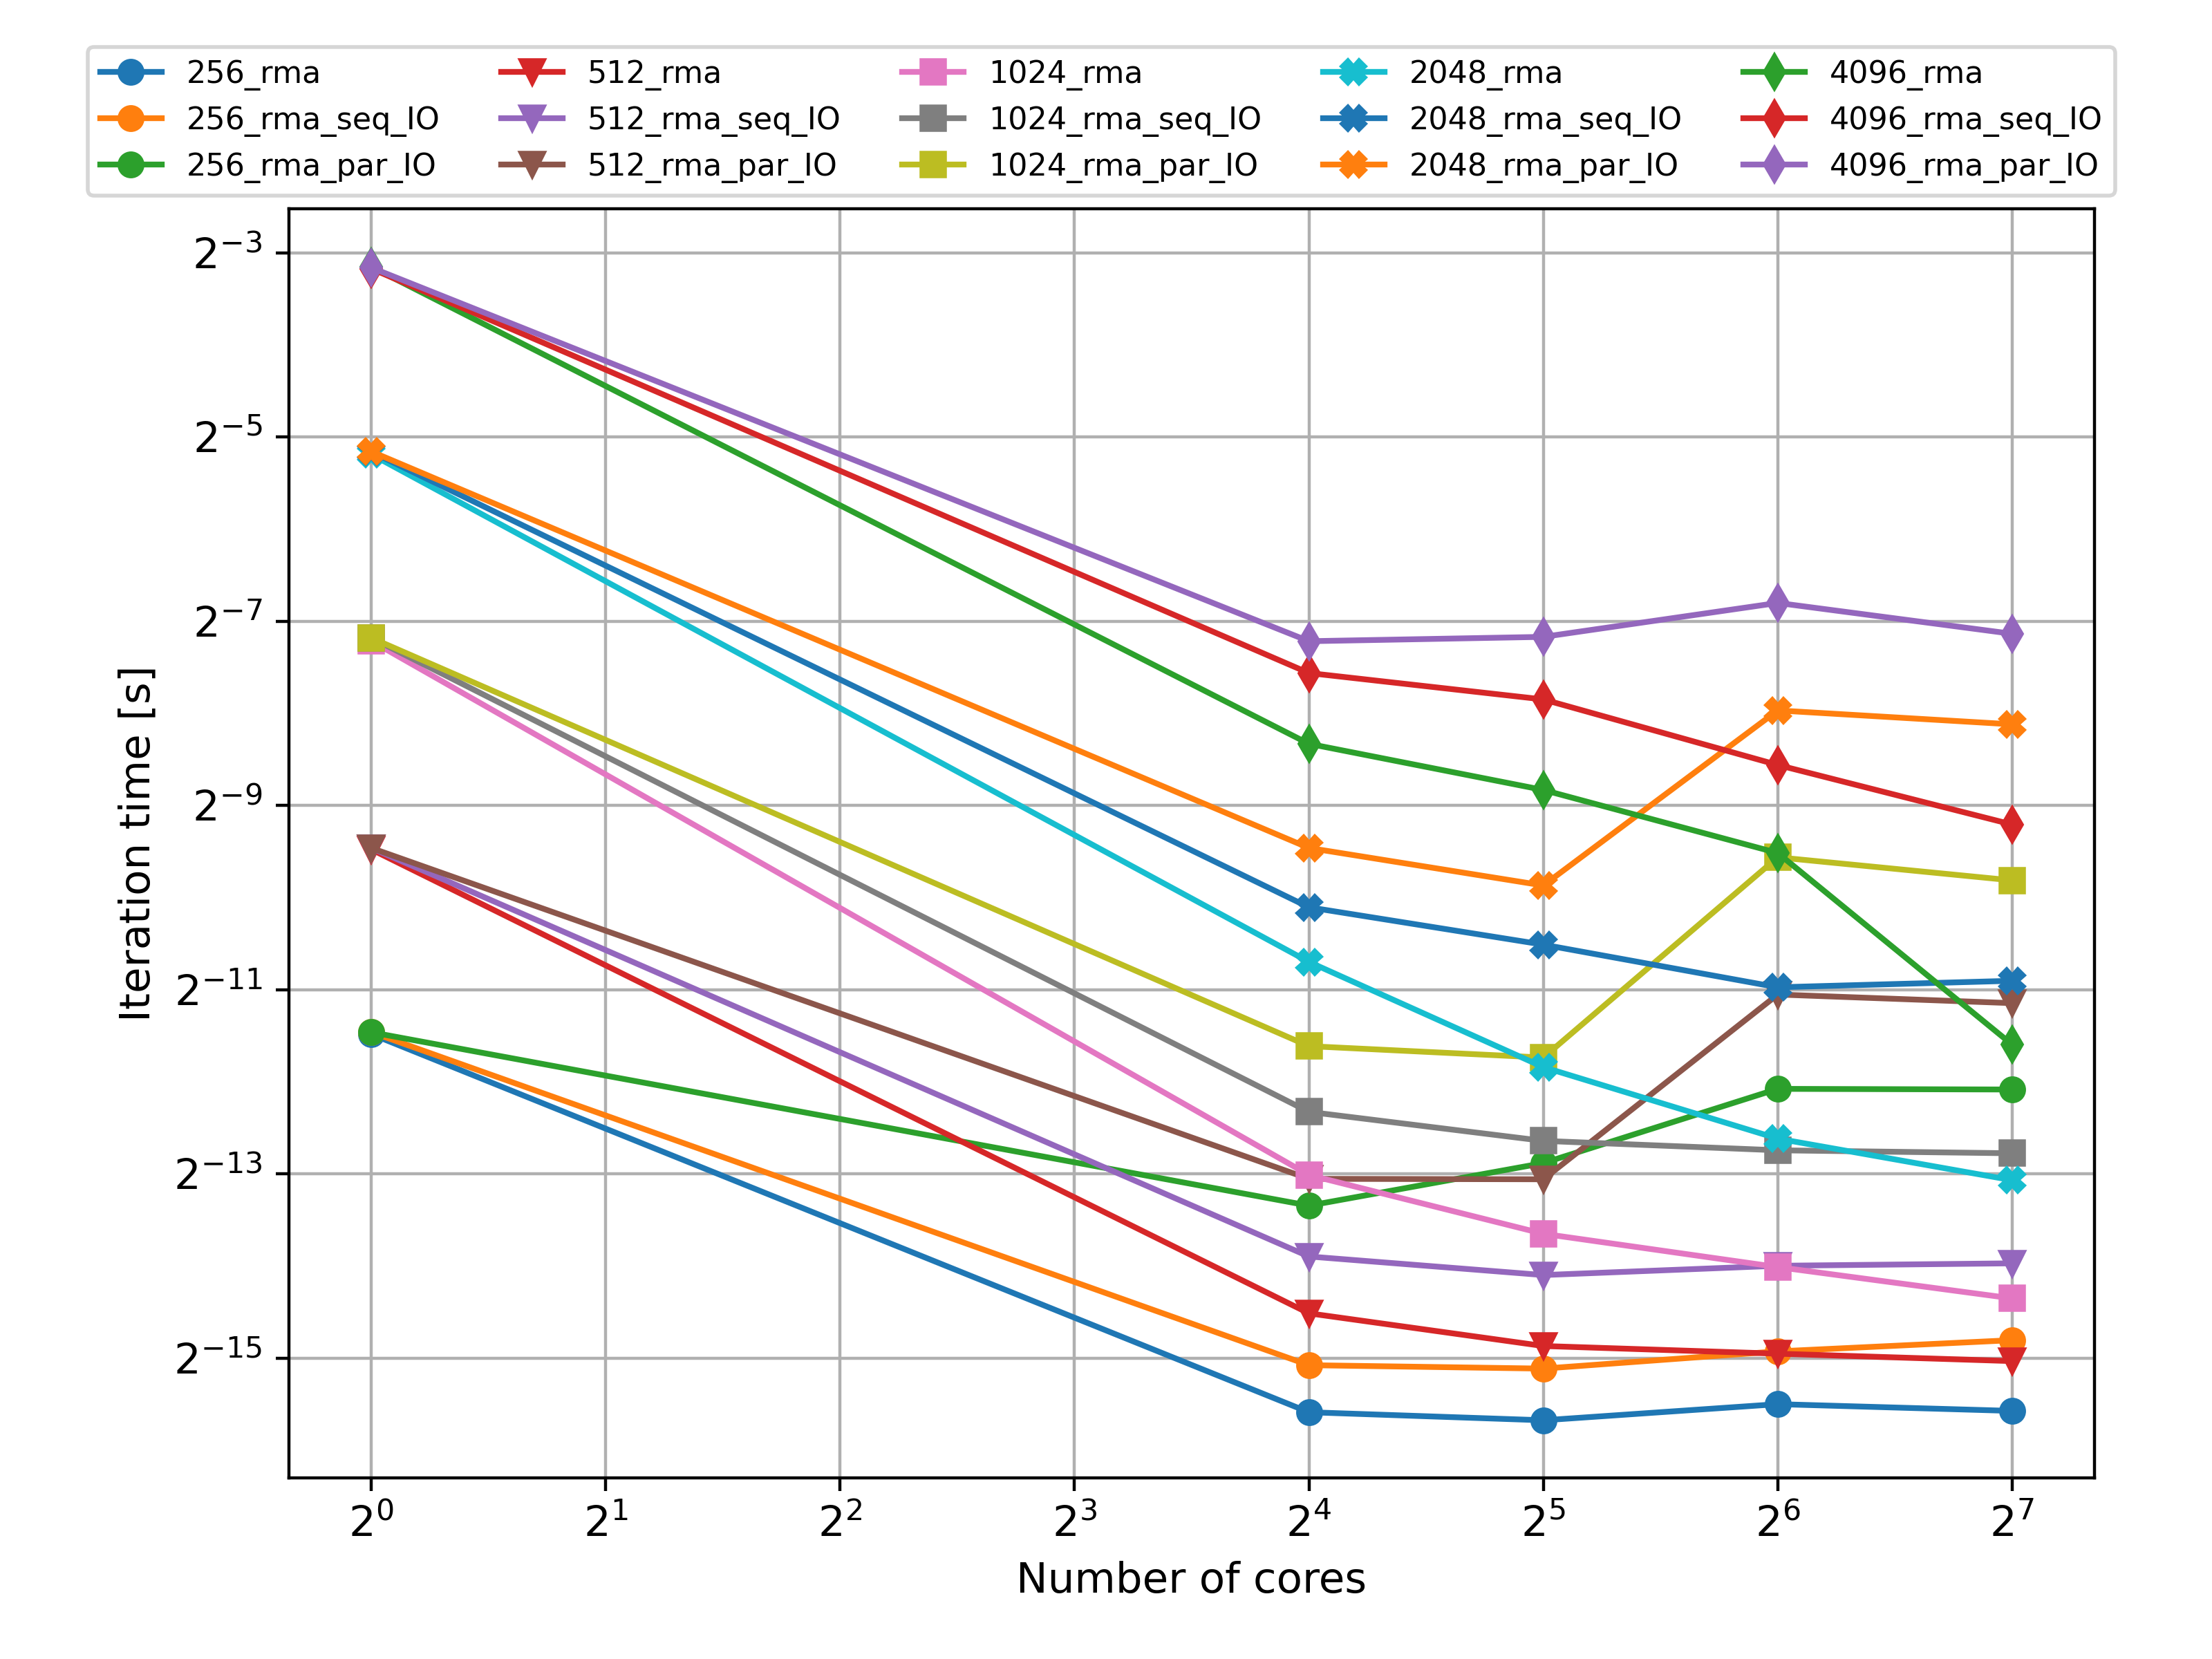
\includegraphics[width=\textwidth]{figures/ppp_scaling_mpi_rma.png}
        \caption{Cena výpočtu: čisté MPI s 2D dekompozicí, RMA.}
        \label{fig:2D_MPI_RMA_eff}
    \end{subfigure}
    \caption{Silné škálování a cena výpočtu: čisté MPI s 2D dekompozicí.}
    \label{fig:2D_MPI}
\end{figure}

% ----- Hybrid 2D -----
\begin{figure}[H]
    \centering
    \begin{subfigure}{0.45\textwidth}
        \centering
        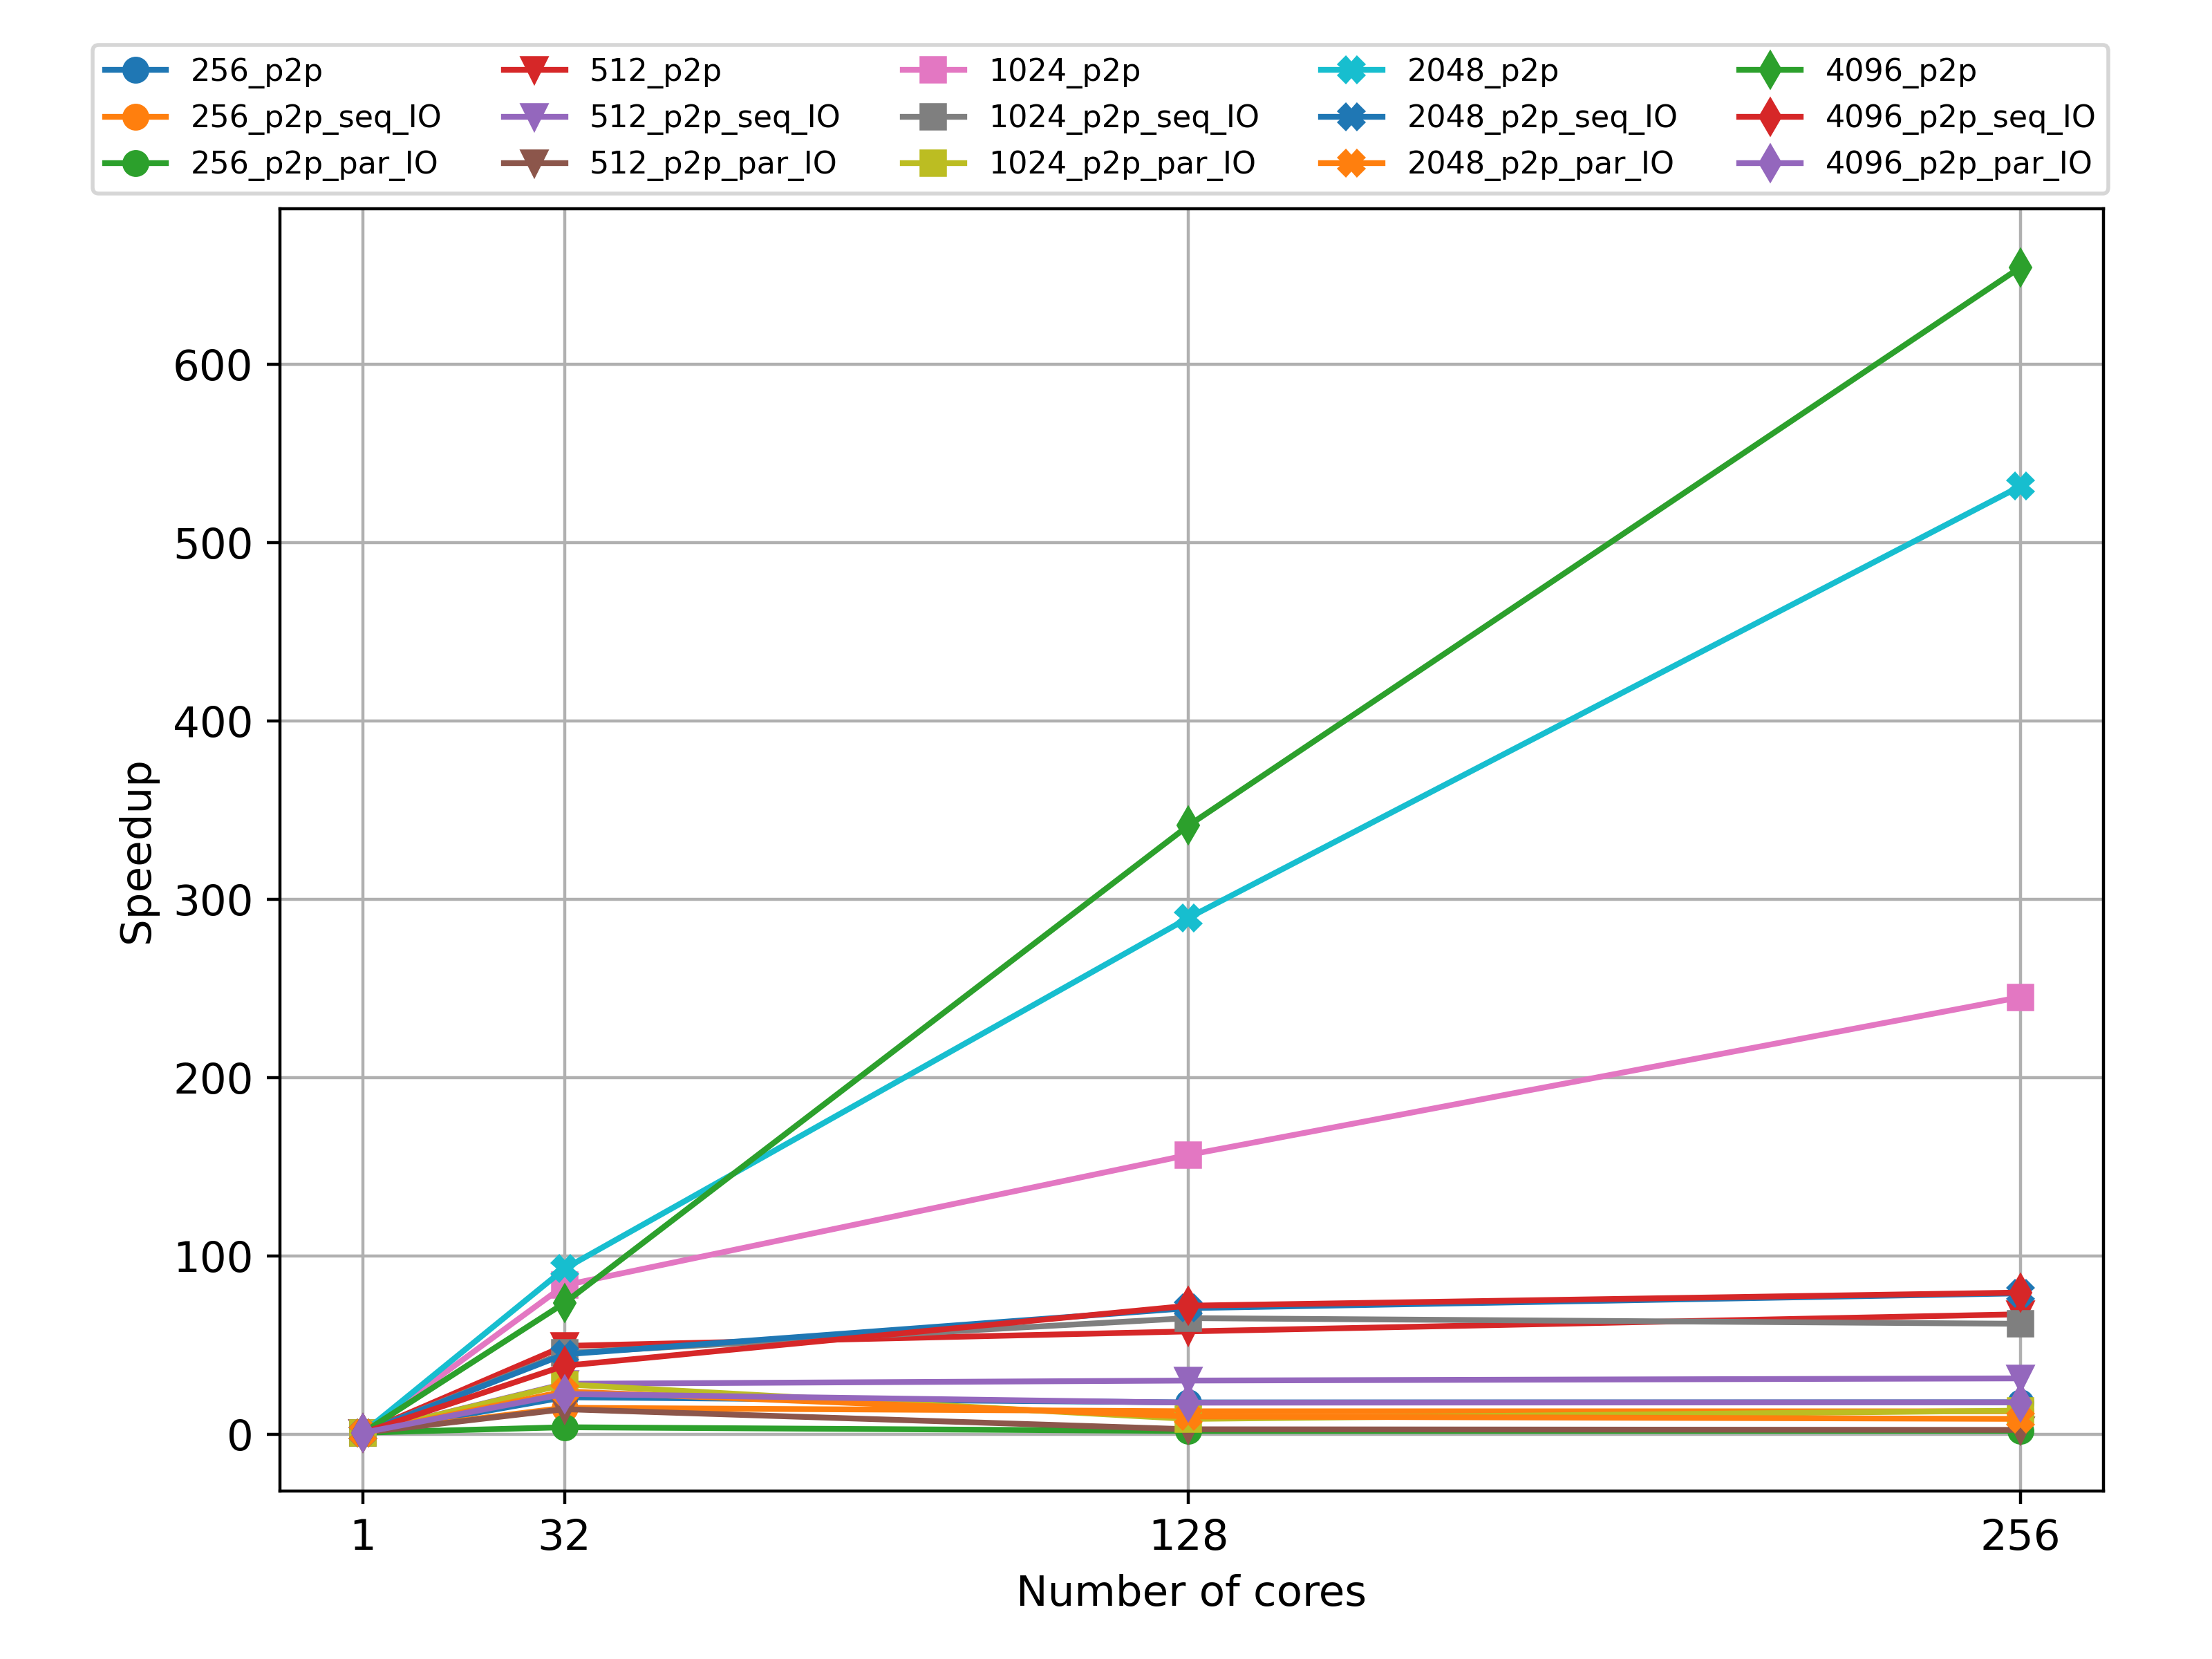
\includegraphics[width=\textwidth]{figures/ppp_speedup_hybrid_p2p.png}
        \caption{Silné škálování: hybridní MPI s 2D dekompozicí, P2P.}
        \label{fig:2D_hybrid_P2P}
    \end{subfigure}
    \hfill
    \begin{subfigure}{0.45\textwidth}
        \centering
        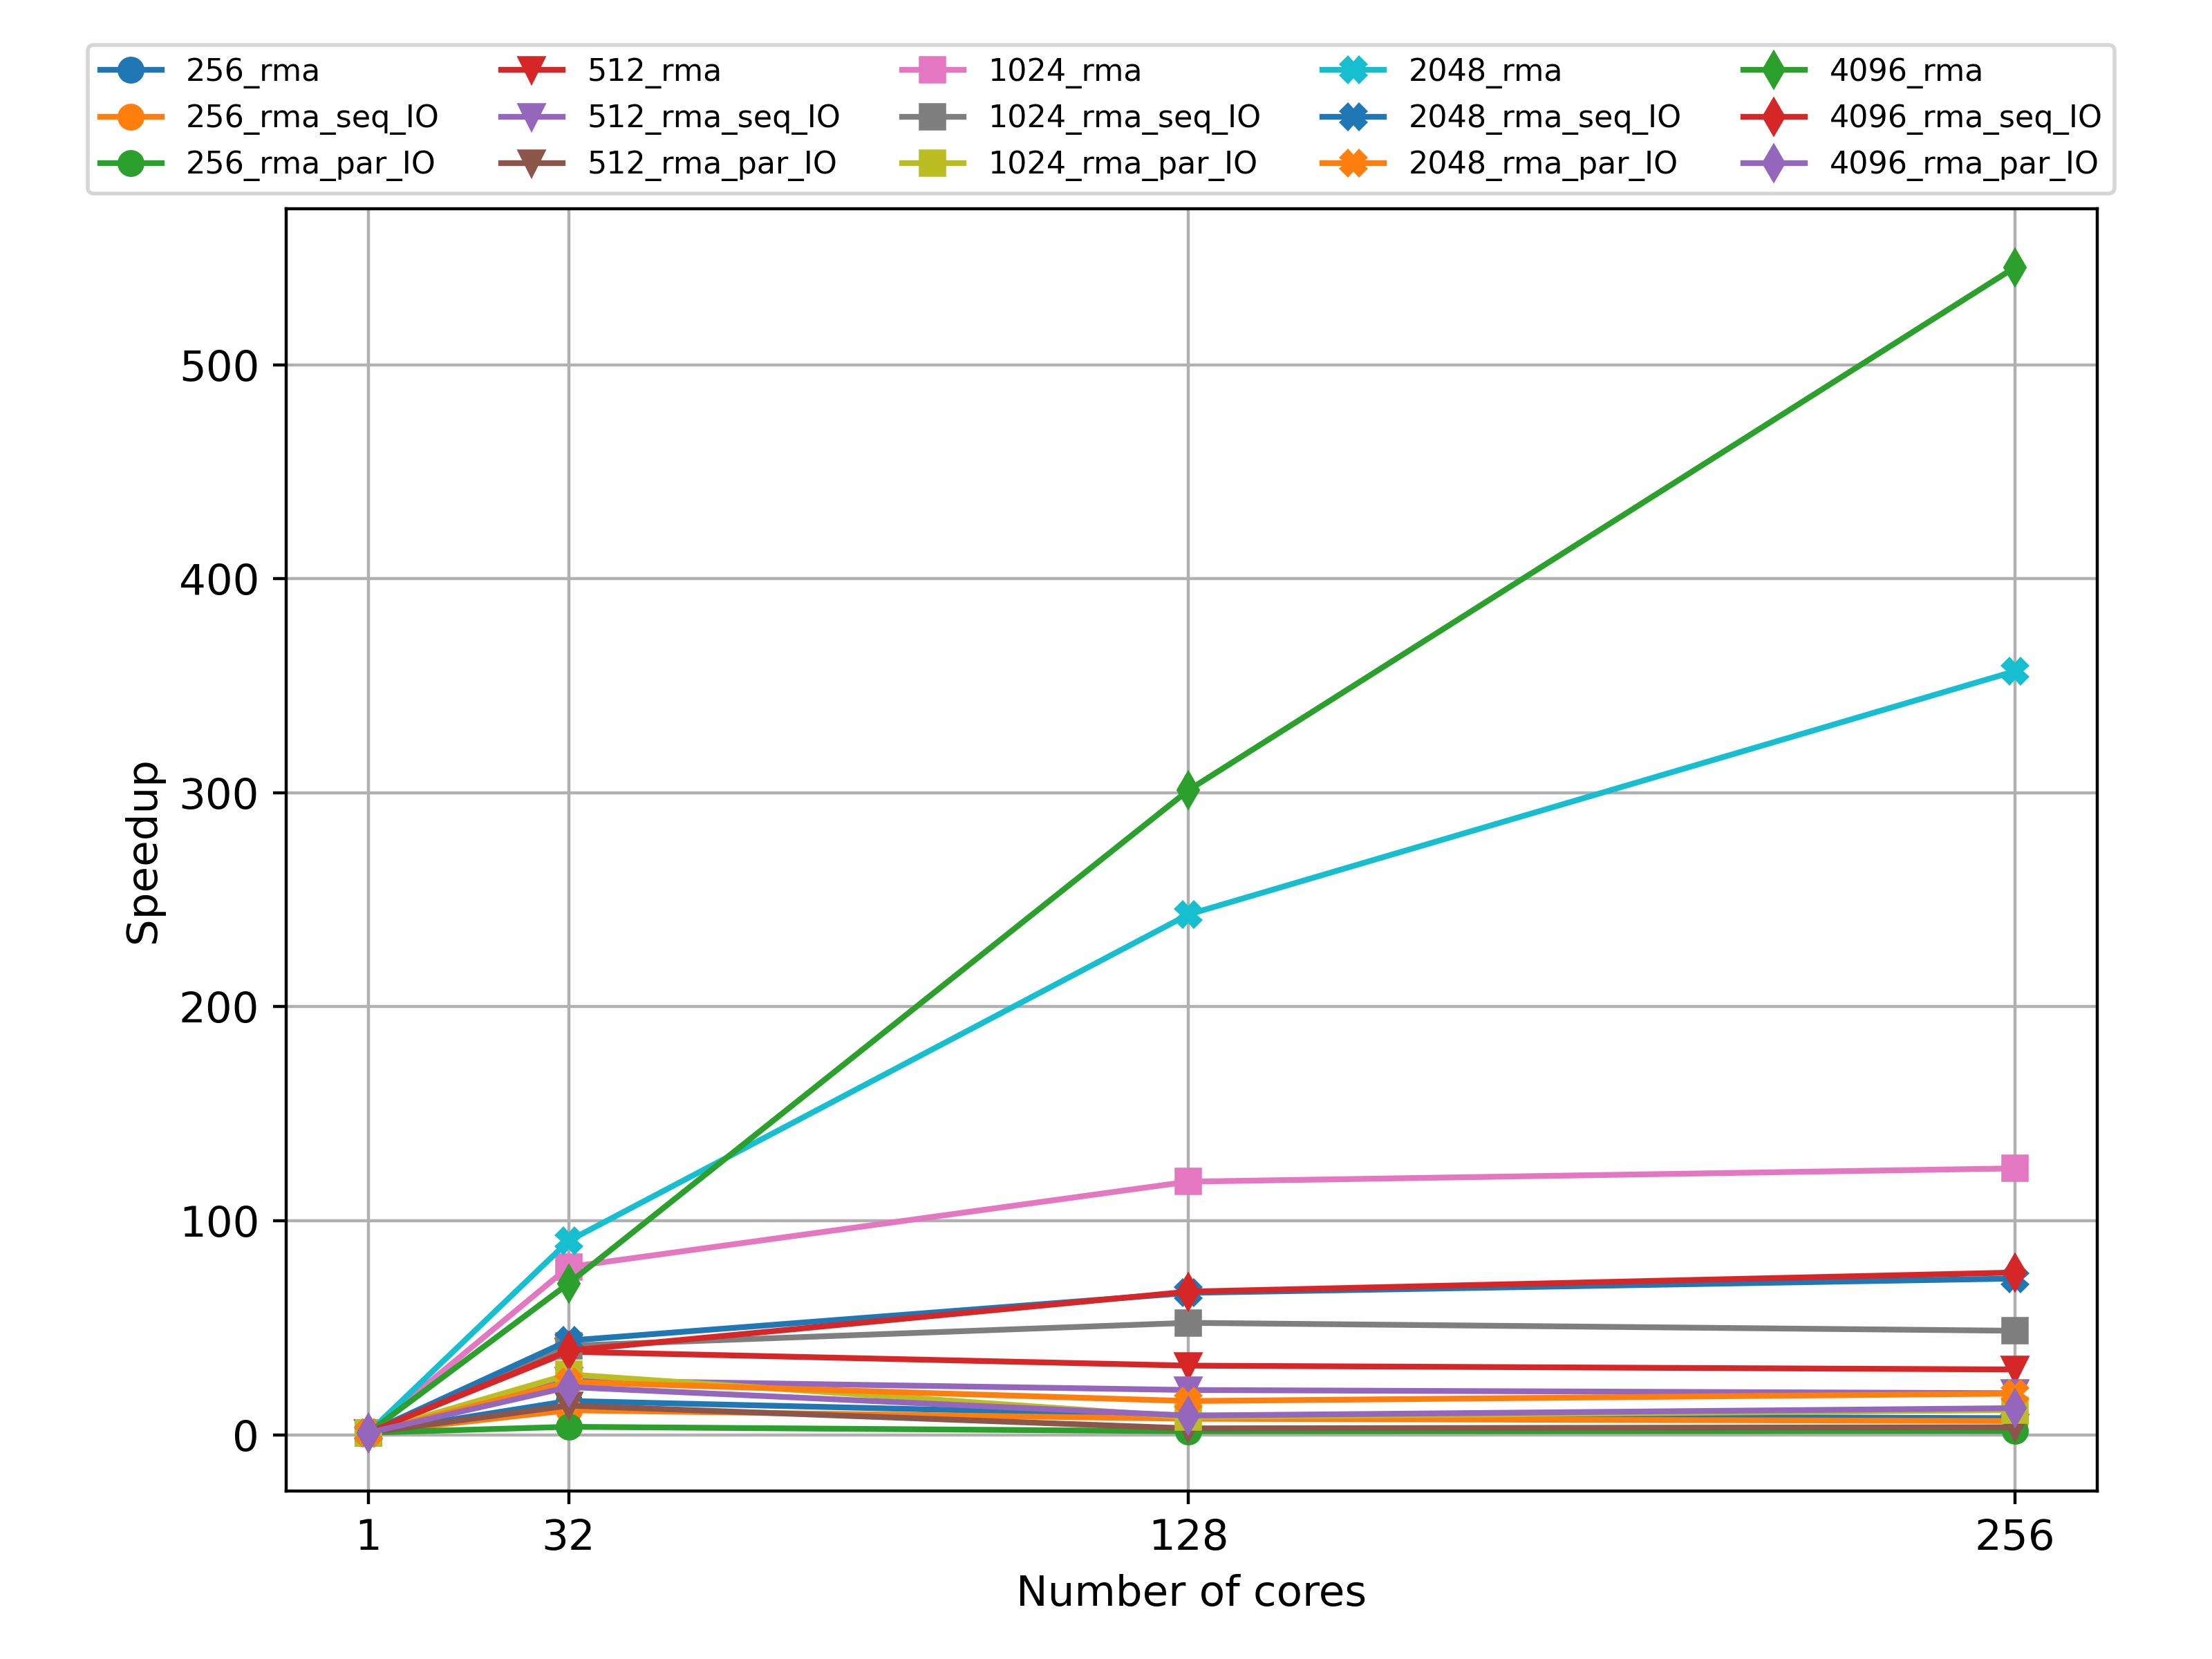
\includegraphics[width=\textwidth]{figures/ppp_speedup_hybrid_rma.png}
        \caption{Silné škálování: hybridní MPI s 2D dekompozicí, RMA.}
        \label{fig:2D_hybrid_RMA}
    \end{subfigure}

    \begin{subfigure}{0.45\textwidth}
        \centering
        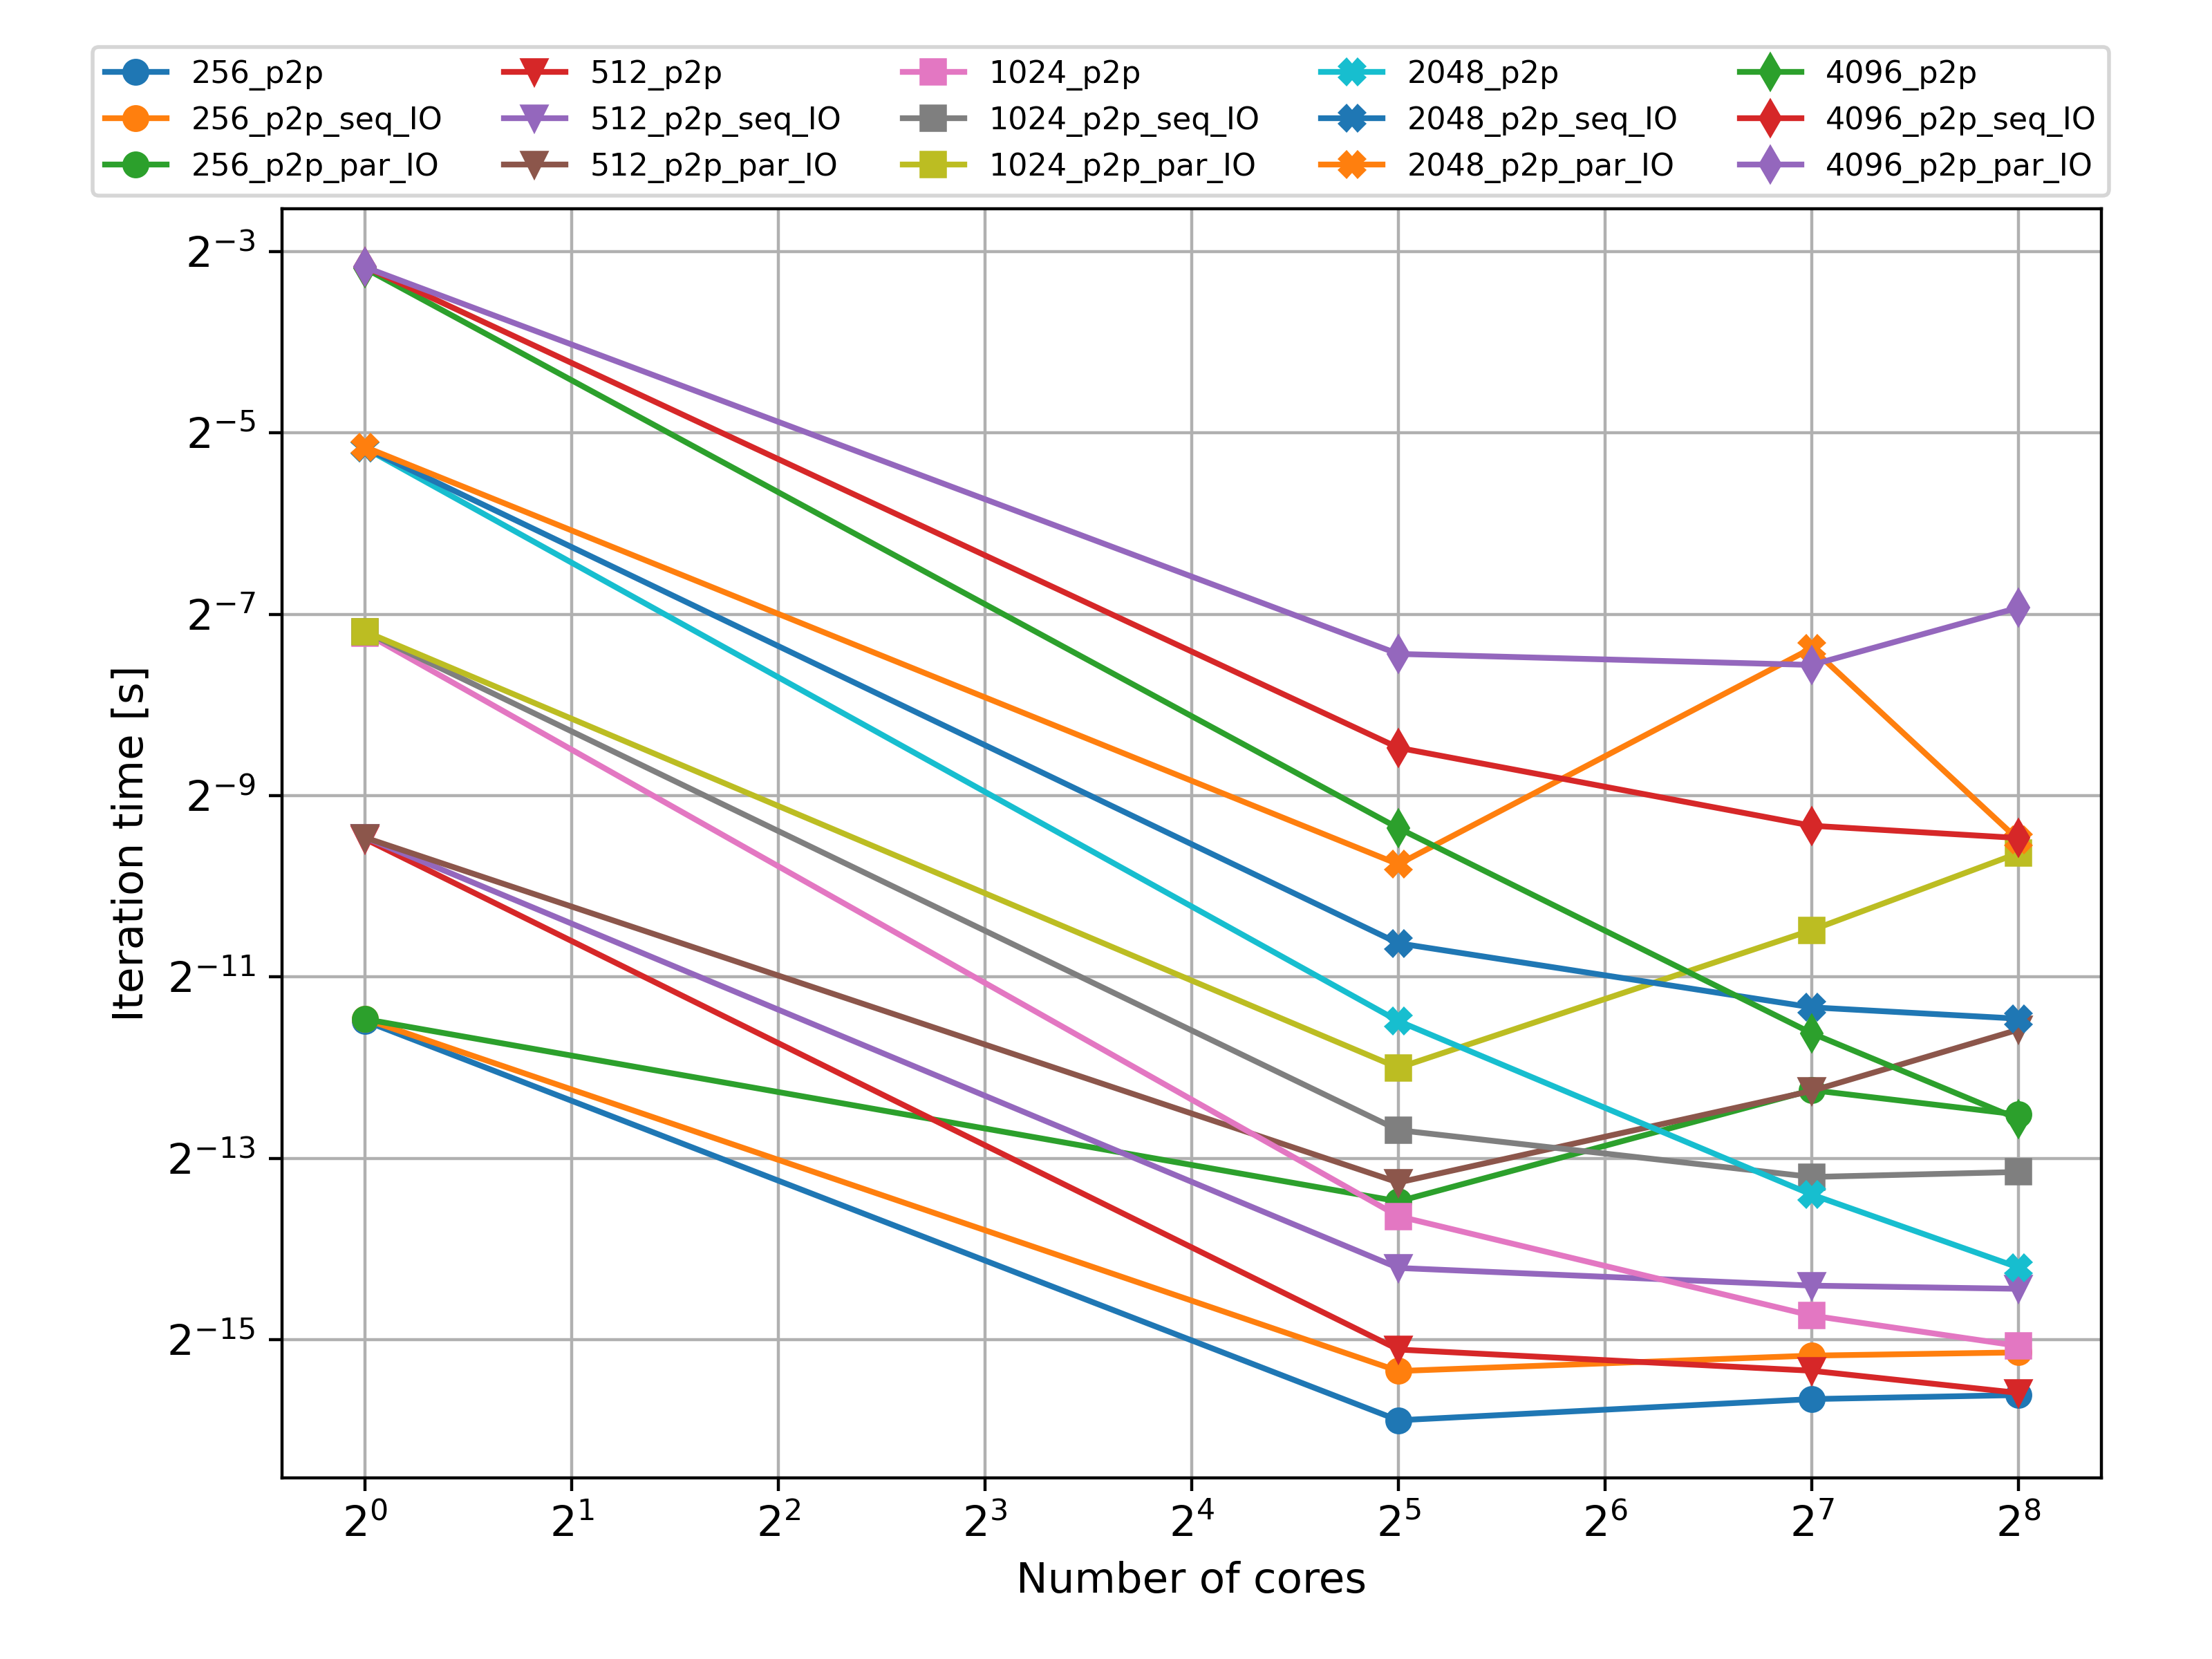
\includegraphics[width=\textwidth]{figures/ppp_scaling_hybrid_p2p.png}
        \caption{Cena výpočtu: hybridní MPI s 2D dekompozicí, P2P.}
        \label{fig:2D_hybrid_P2P_eff}
    \end{subfigure}
    \hfill
    \begin{subfigure}{0.45\textwidth}
        \centering
        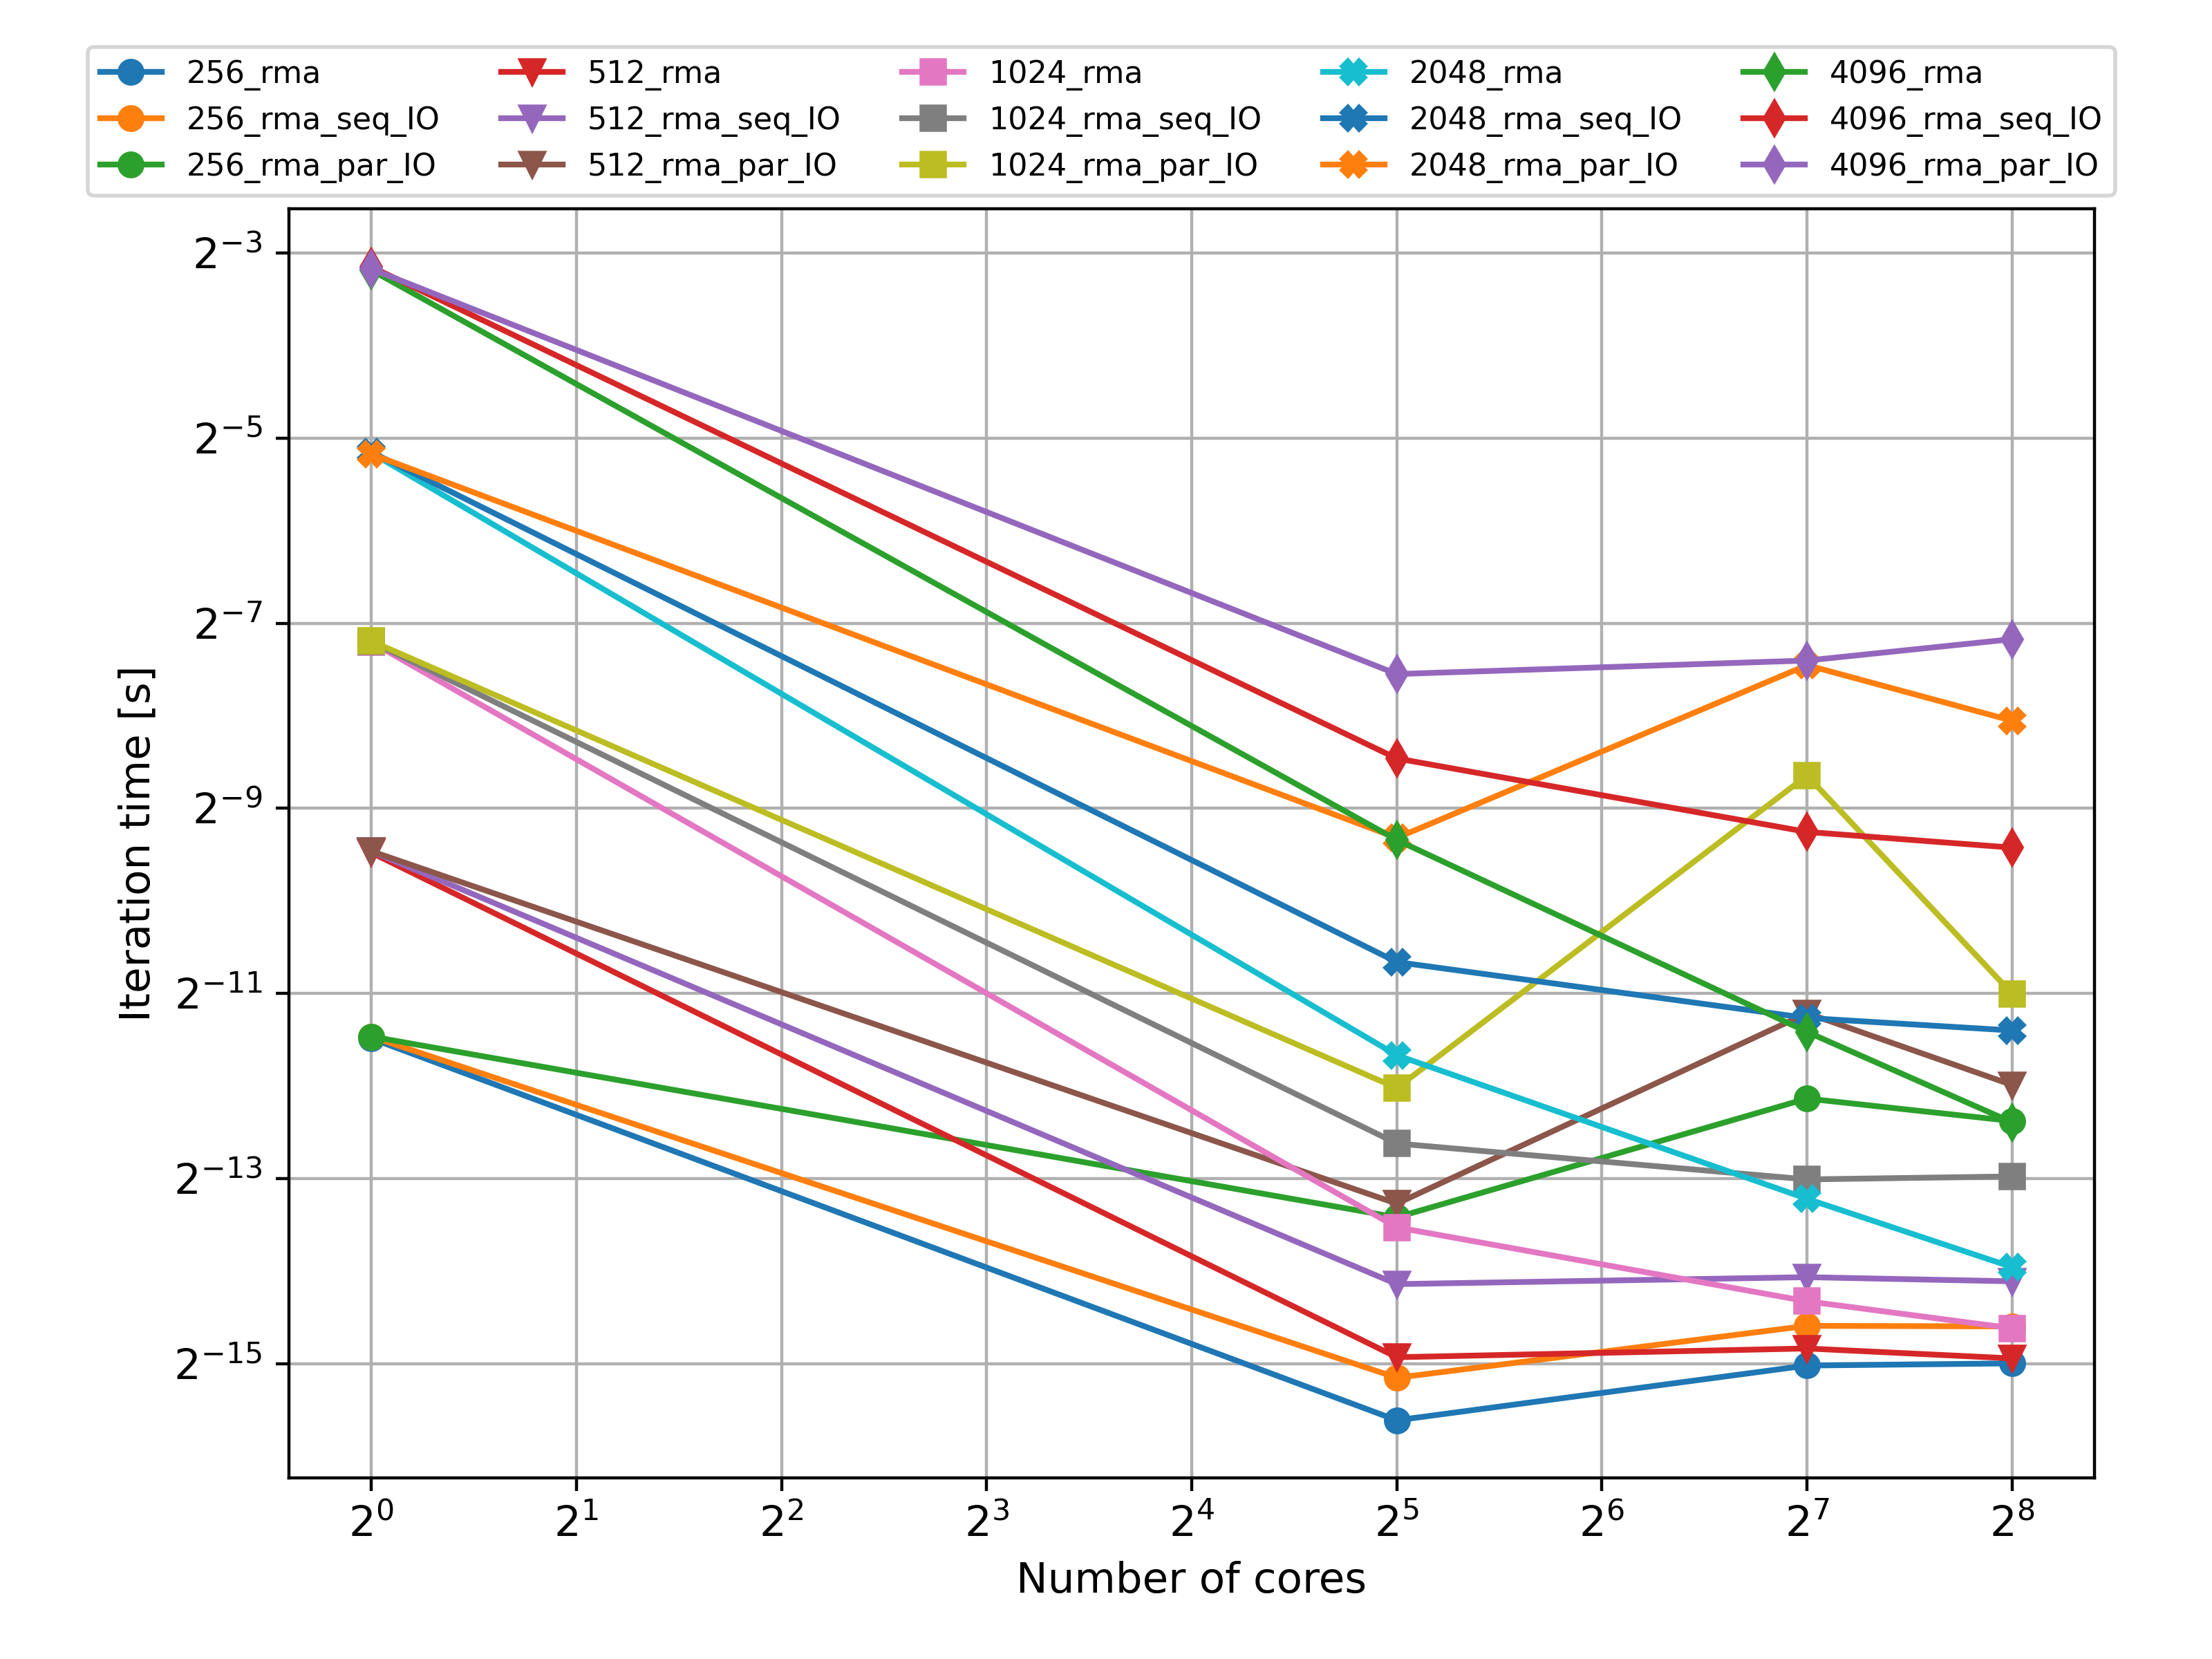
\includegraphics[width=\textwidth]{figures/ppp_scaling_hybrid_rma.png}
        \caption{Cena výpočtu: hybridní MPI s 2D dekompozicí, RMA.}
        \label{fig:2D_hybrid_RMA_eff}
    \end{subfigure}
    \caption{Silné škálování a cena výpočtu: hybridní MPI s 2D dekompozicí.}
    \label{fig:2D_hybrid}
\end{figure}

% ----- Hybrid 1D -----
\begin{figure}[H]
    \centering
    \begin{subfigure}{0.45\textwidth}
        \centering
        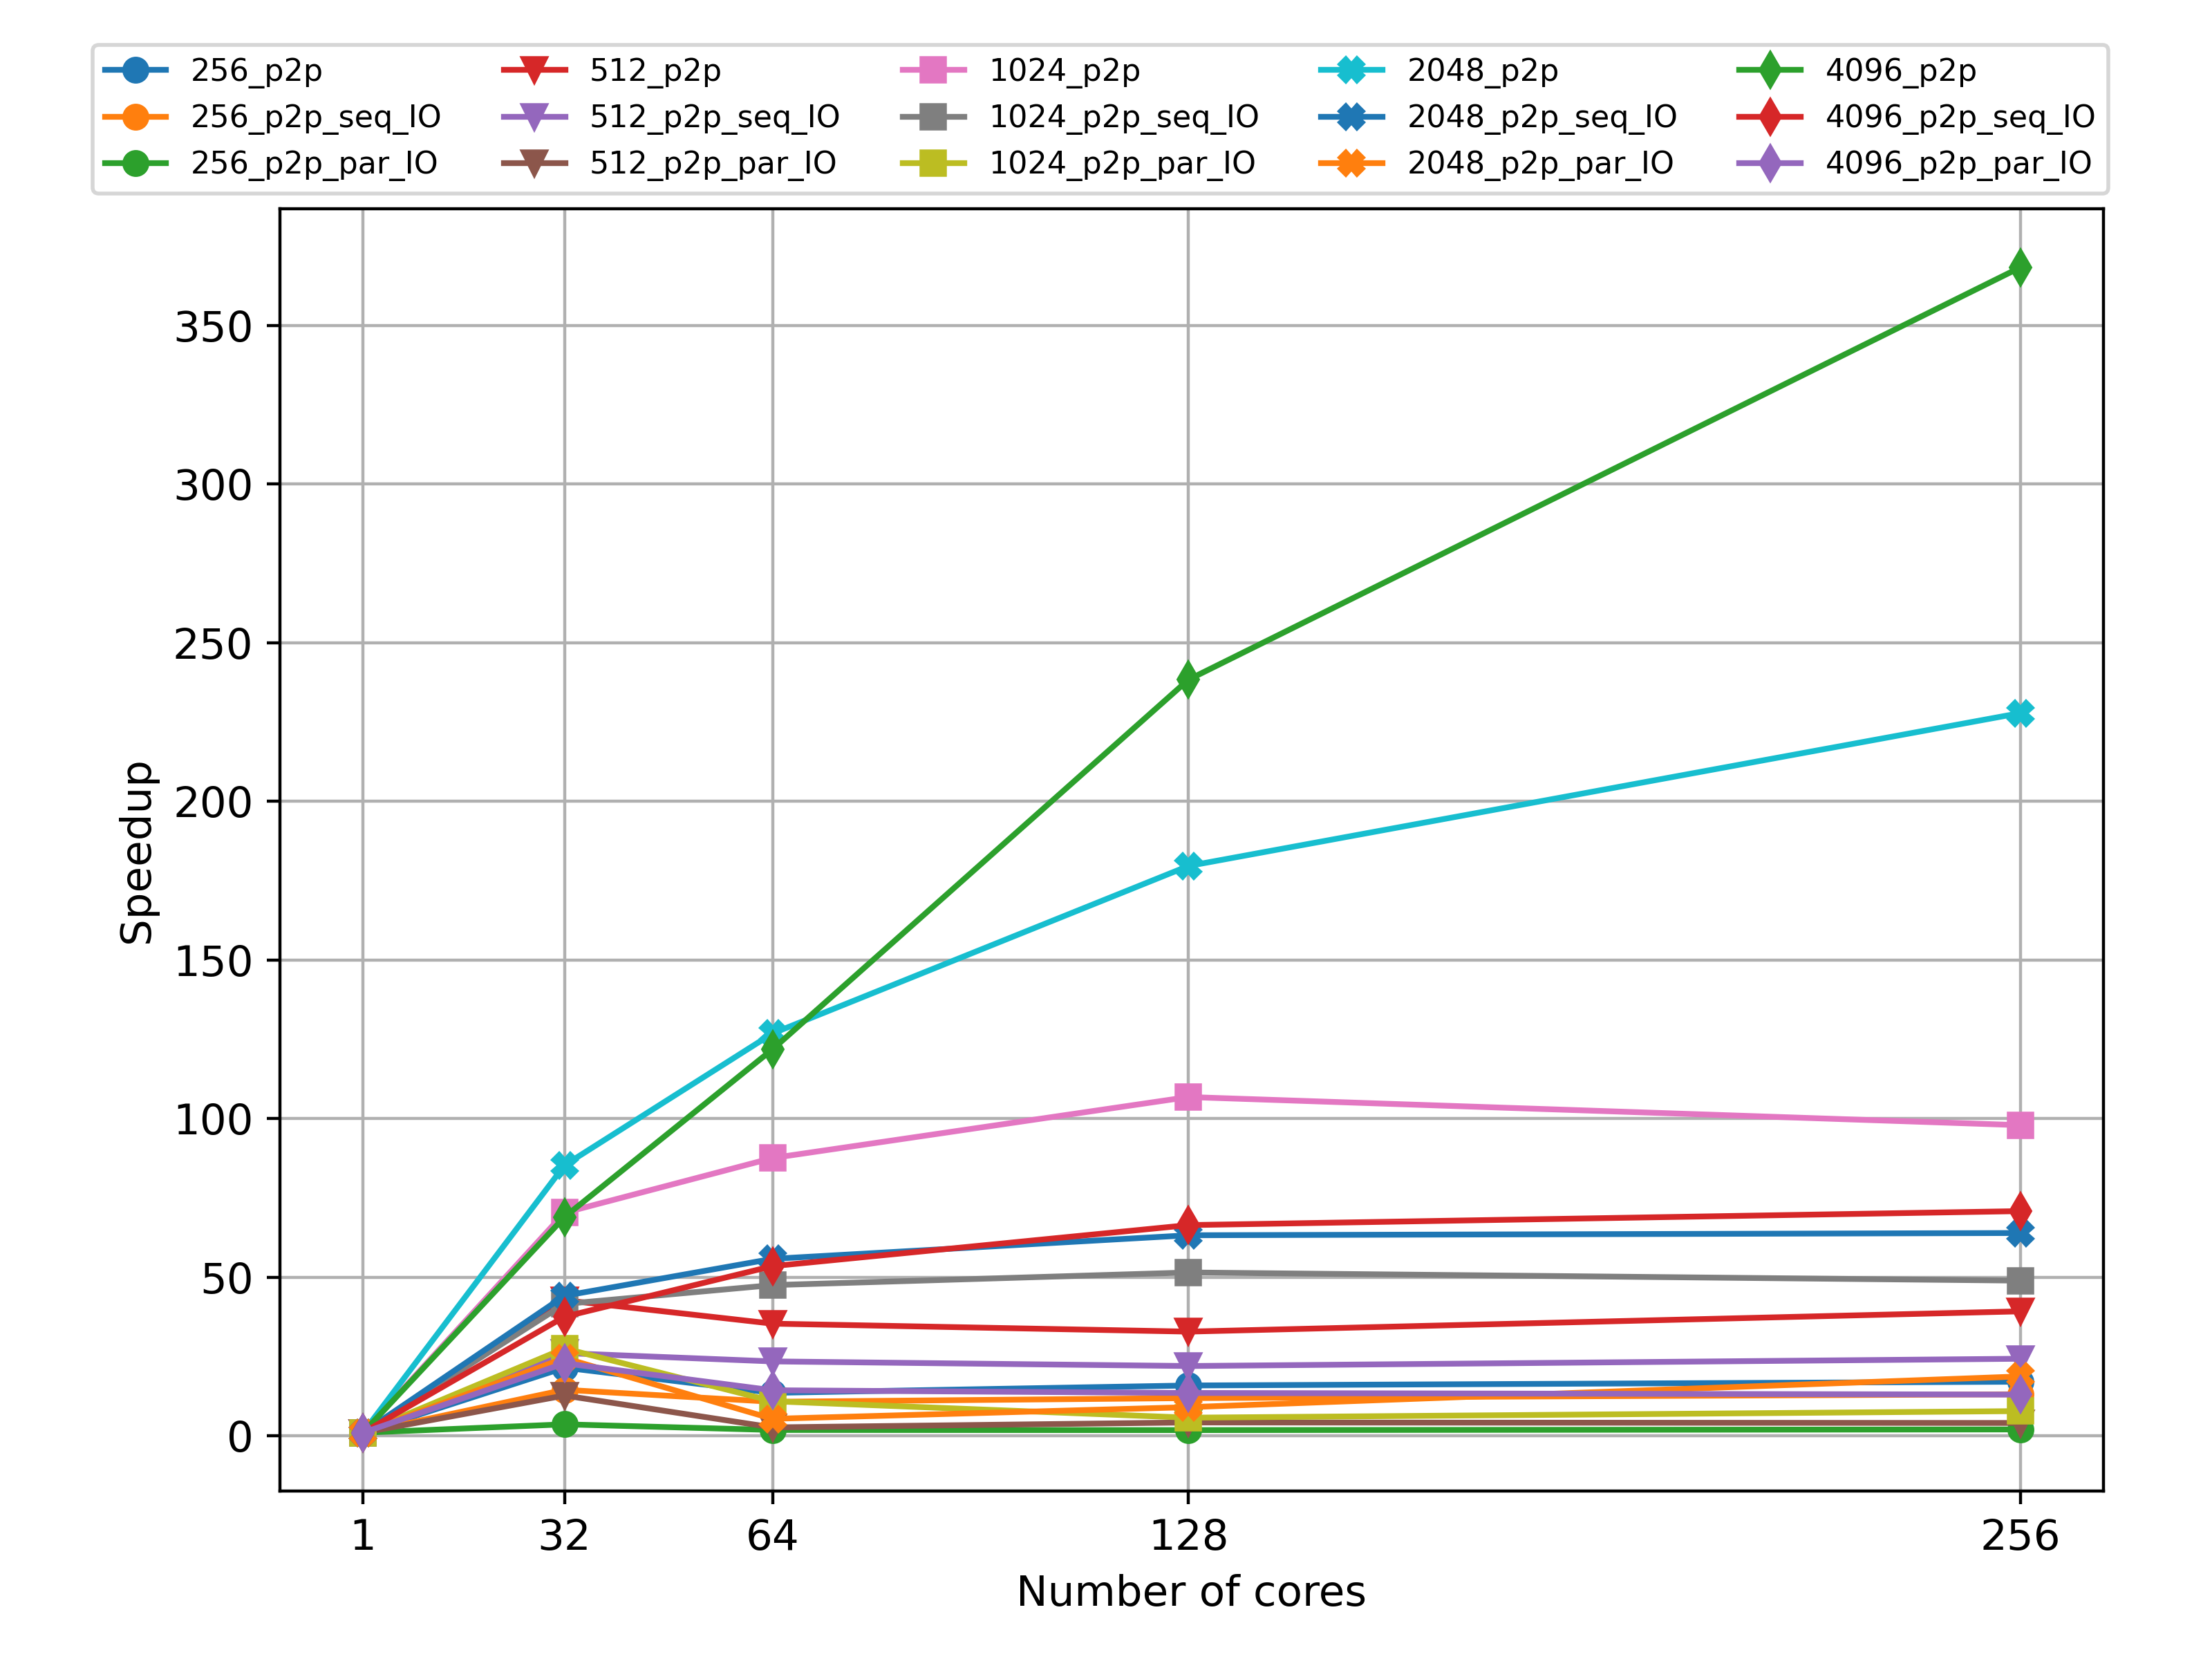
\includegraphics[width=\textwidth]{figures/ppp_speedup_hybrid_1D_p2p.png}
        \caption{Silné škálování: hybridní MPI s 1D dekompozicí, P2P.}
        \label{fig:1D_hybrid_P2P}
    \end{subfigure}
    \hfill
    \begin{subfigure}{0.45\textwidth}
        \centering
        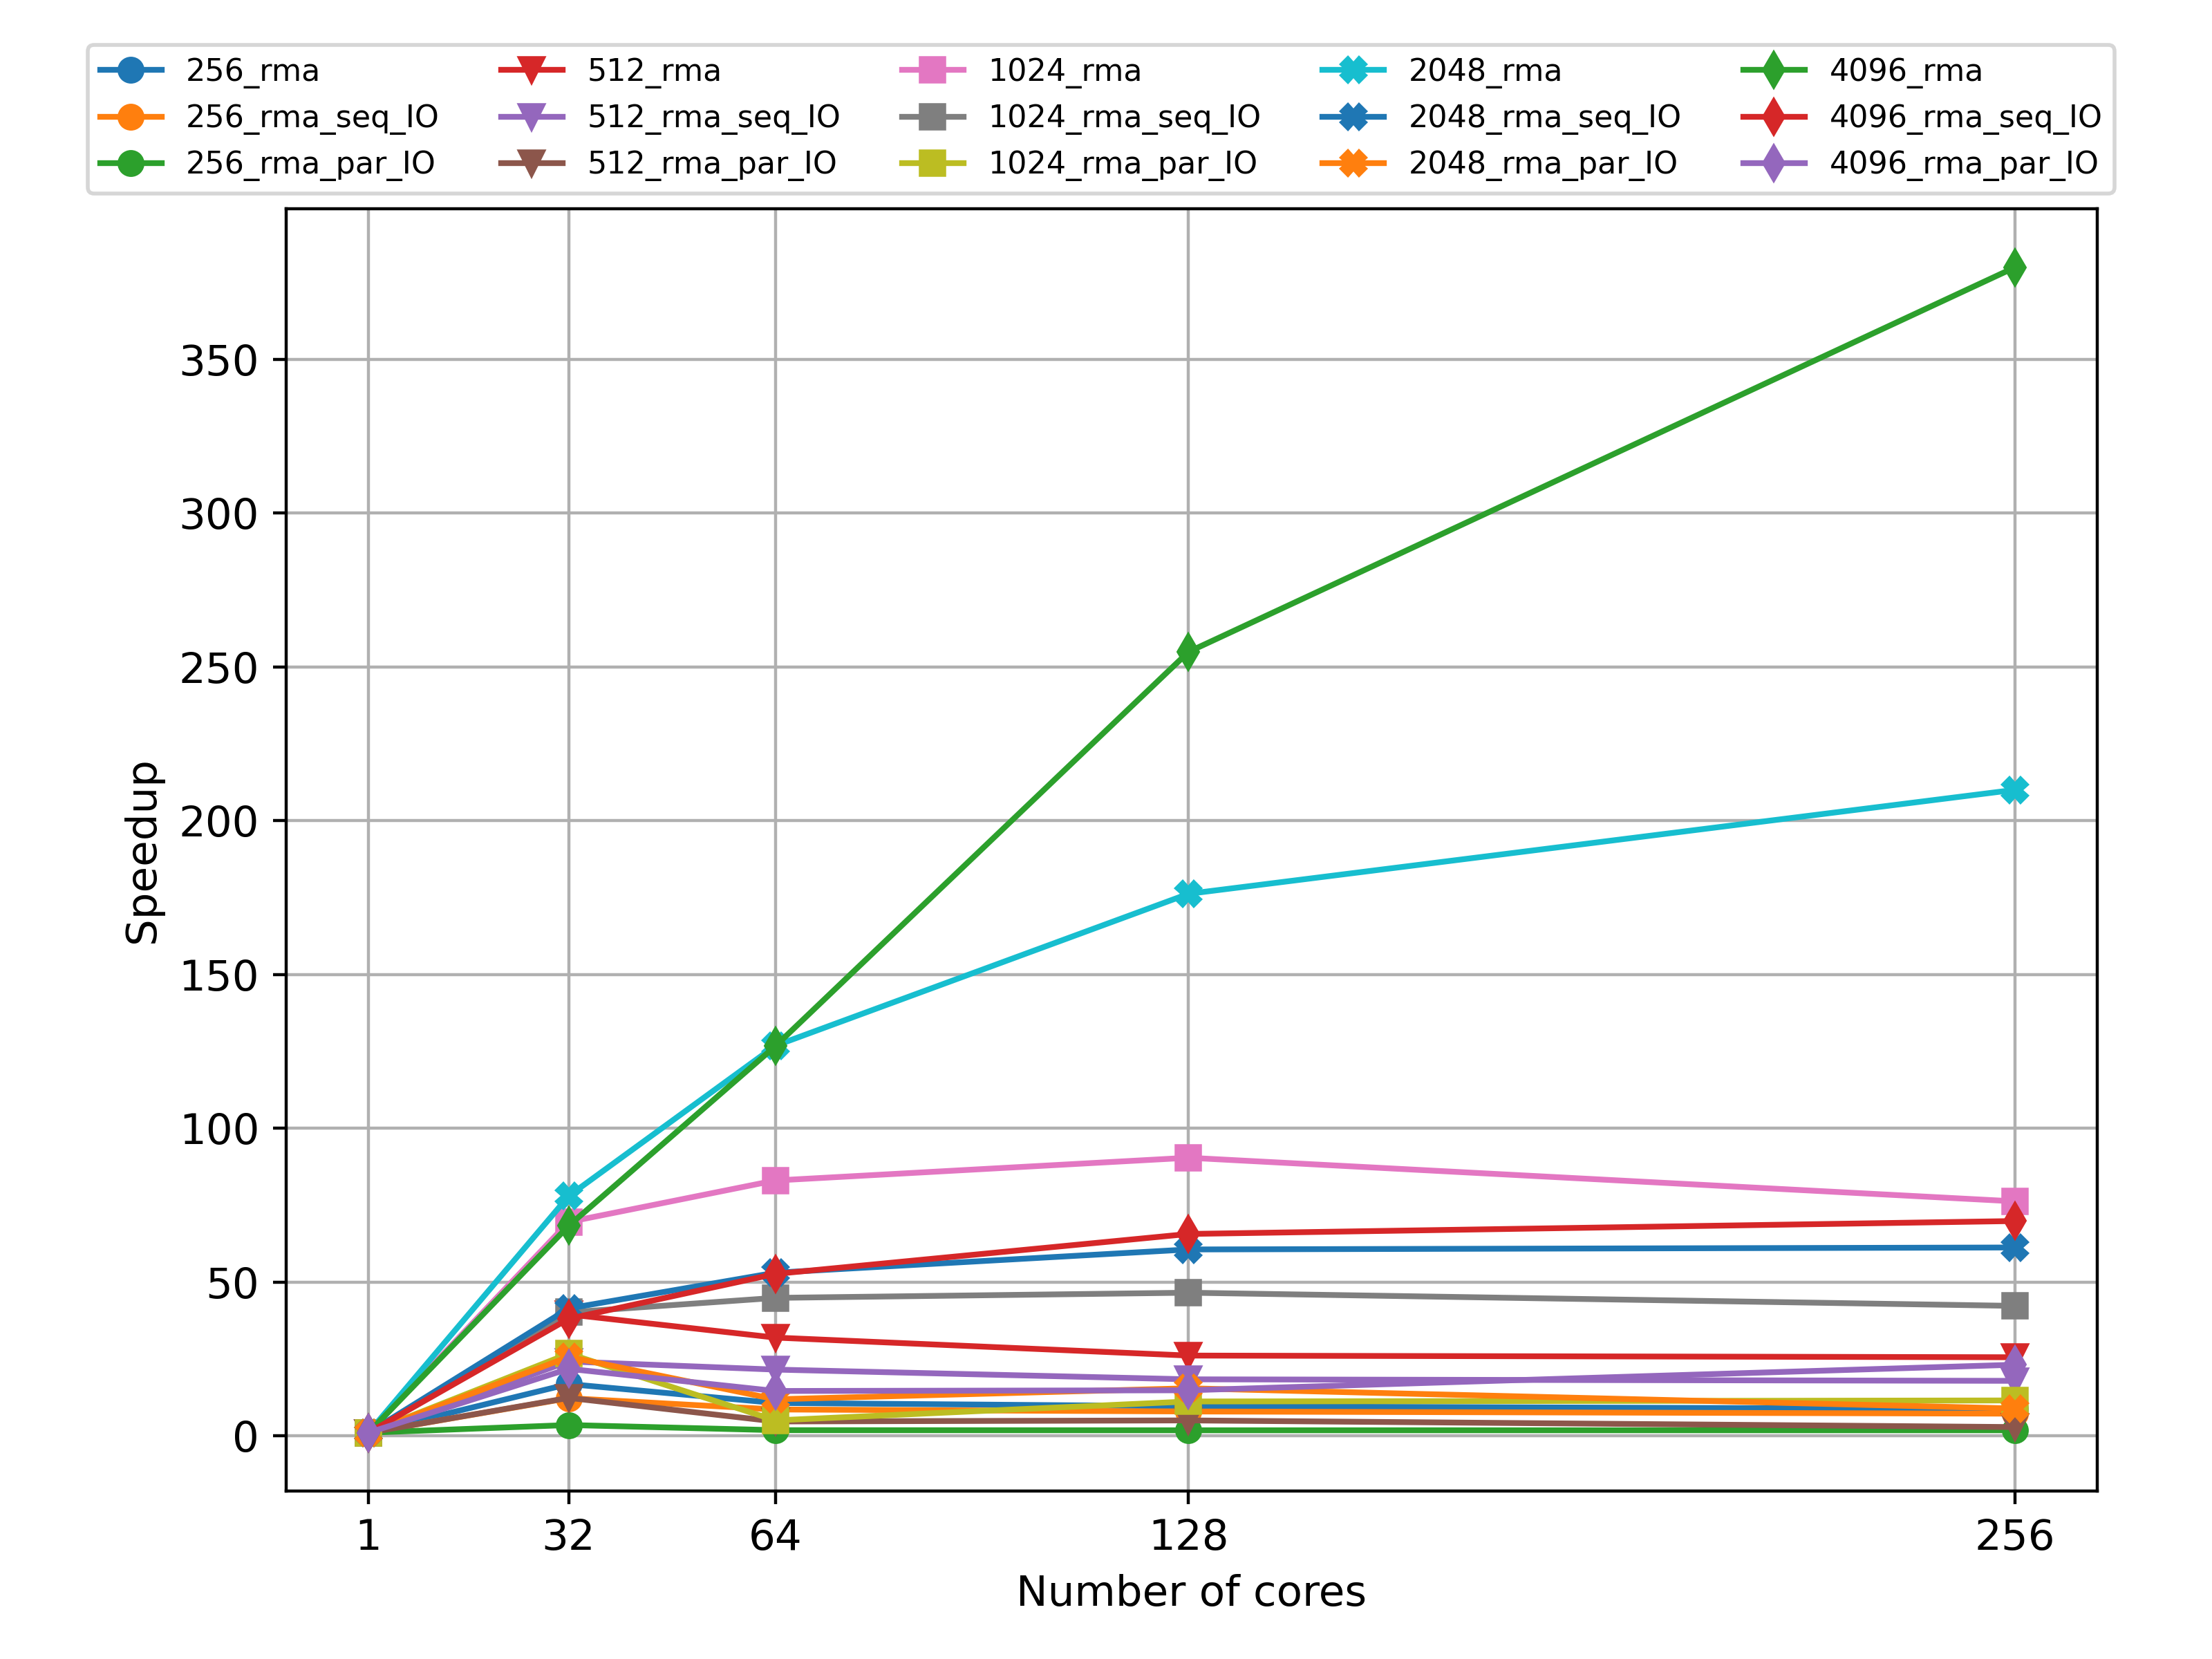
\includegraphics[width=\textwidth]{figures/ppp_speedup_hybrid_1D_rma.png}
        \caption{Silné škálování: hybridní MPI s 1D dekompozicí, RMA.}
        \label{fig:1D_hybrid_RMA}
    \end{subfigure}

    \begin{subfigure}{0.45\textwidth}
        \centering
        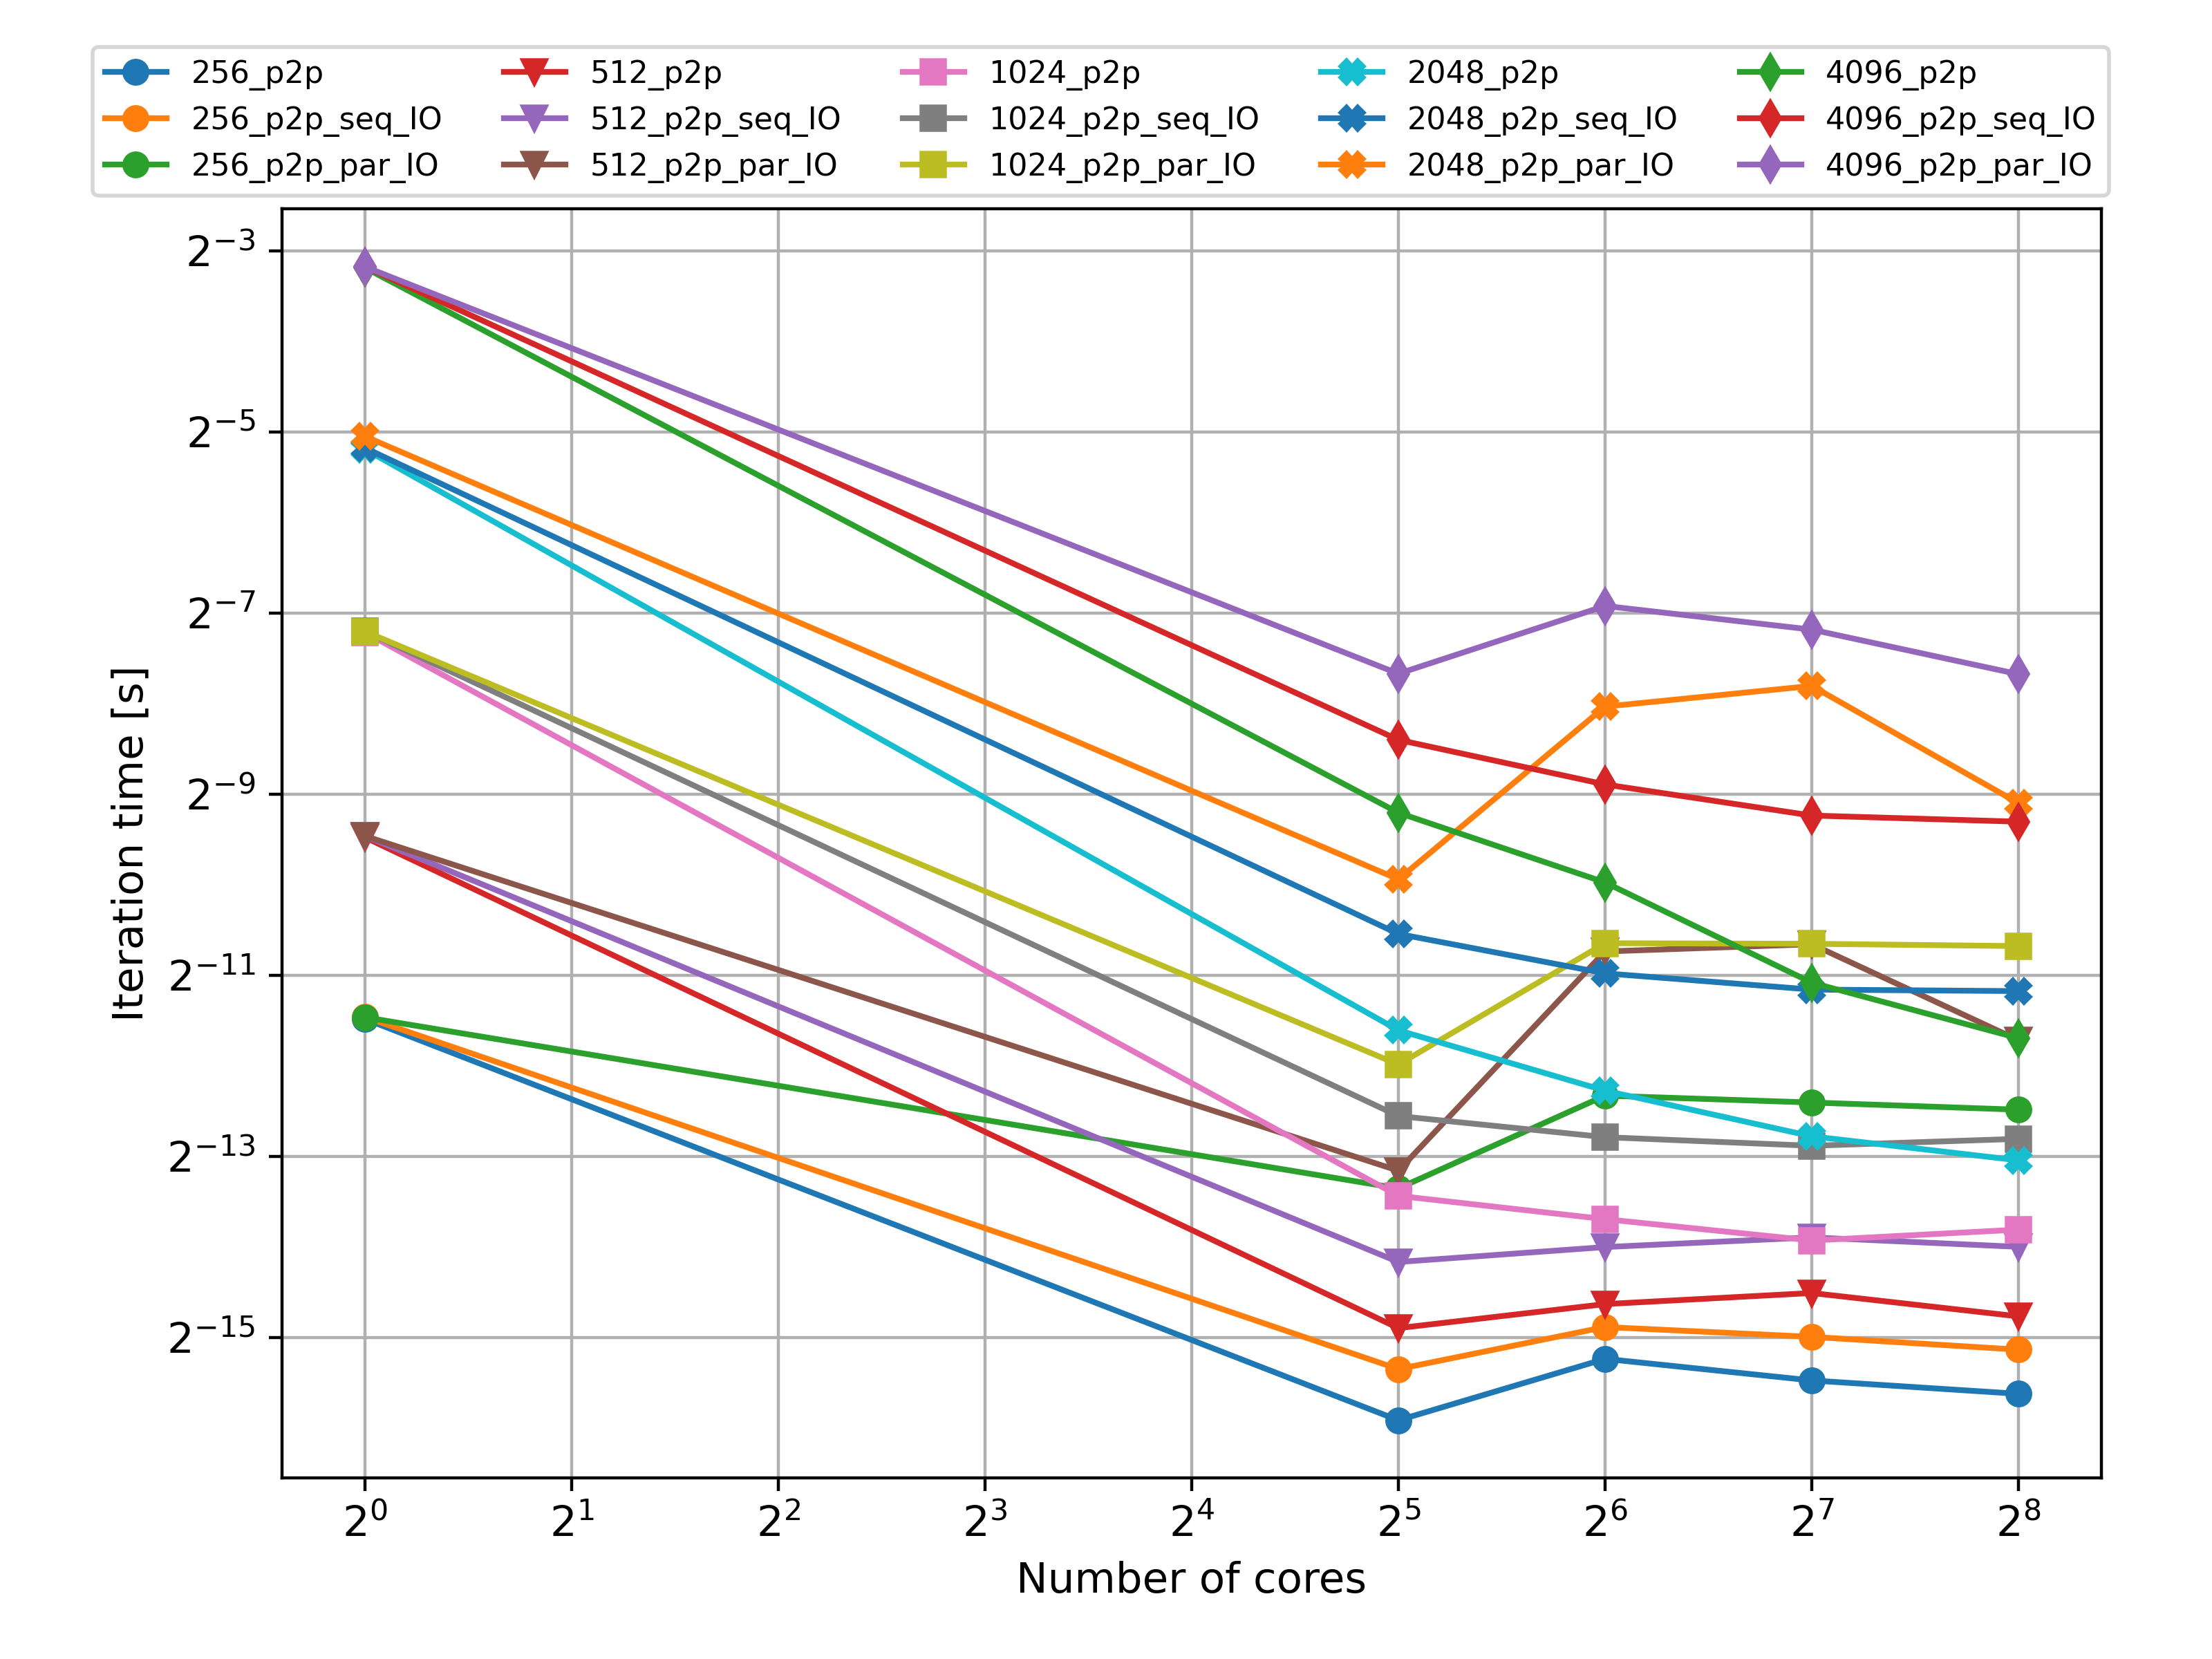
\includegraphics[width=\textwidth]{figures/ppp_scaling_hybrid_1D_p2p.png}
        \caption{Cena výpočtu: hybridní MPI s 1D dekompozicí, P2P.}
        \label{fig:1D_hybrid_P2P_eff}
    \end{subfigure}
    \hfill
    \begin{subfigure}{0.45\textwidth}
        \centering
        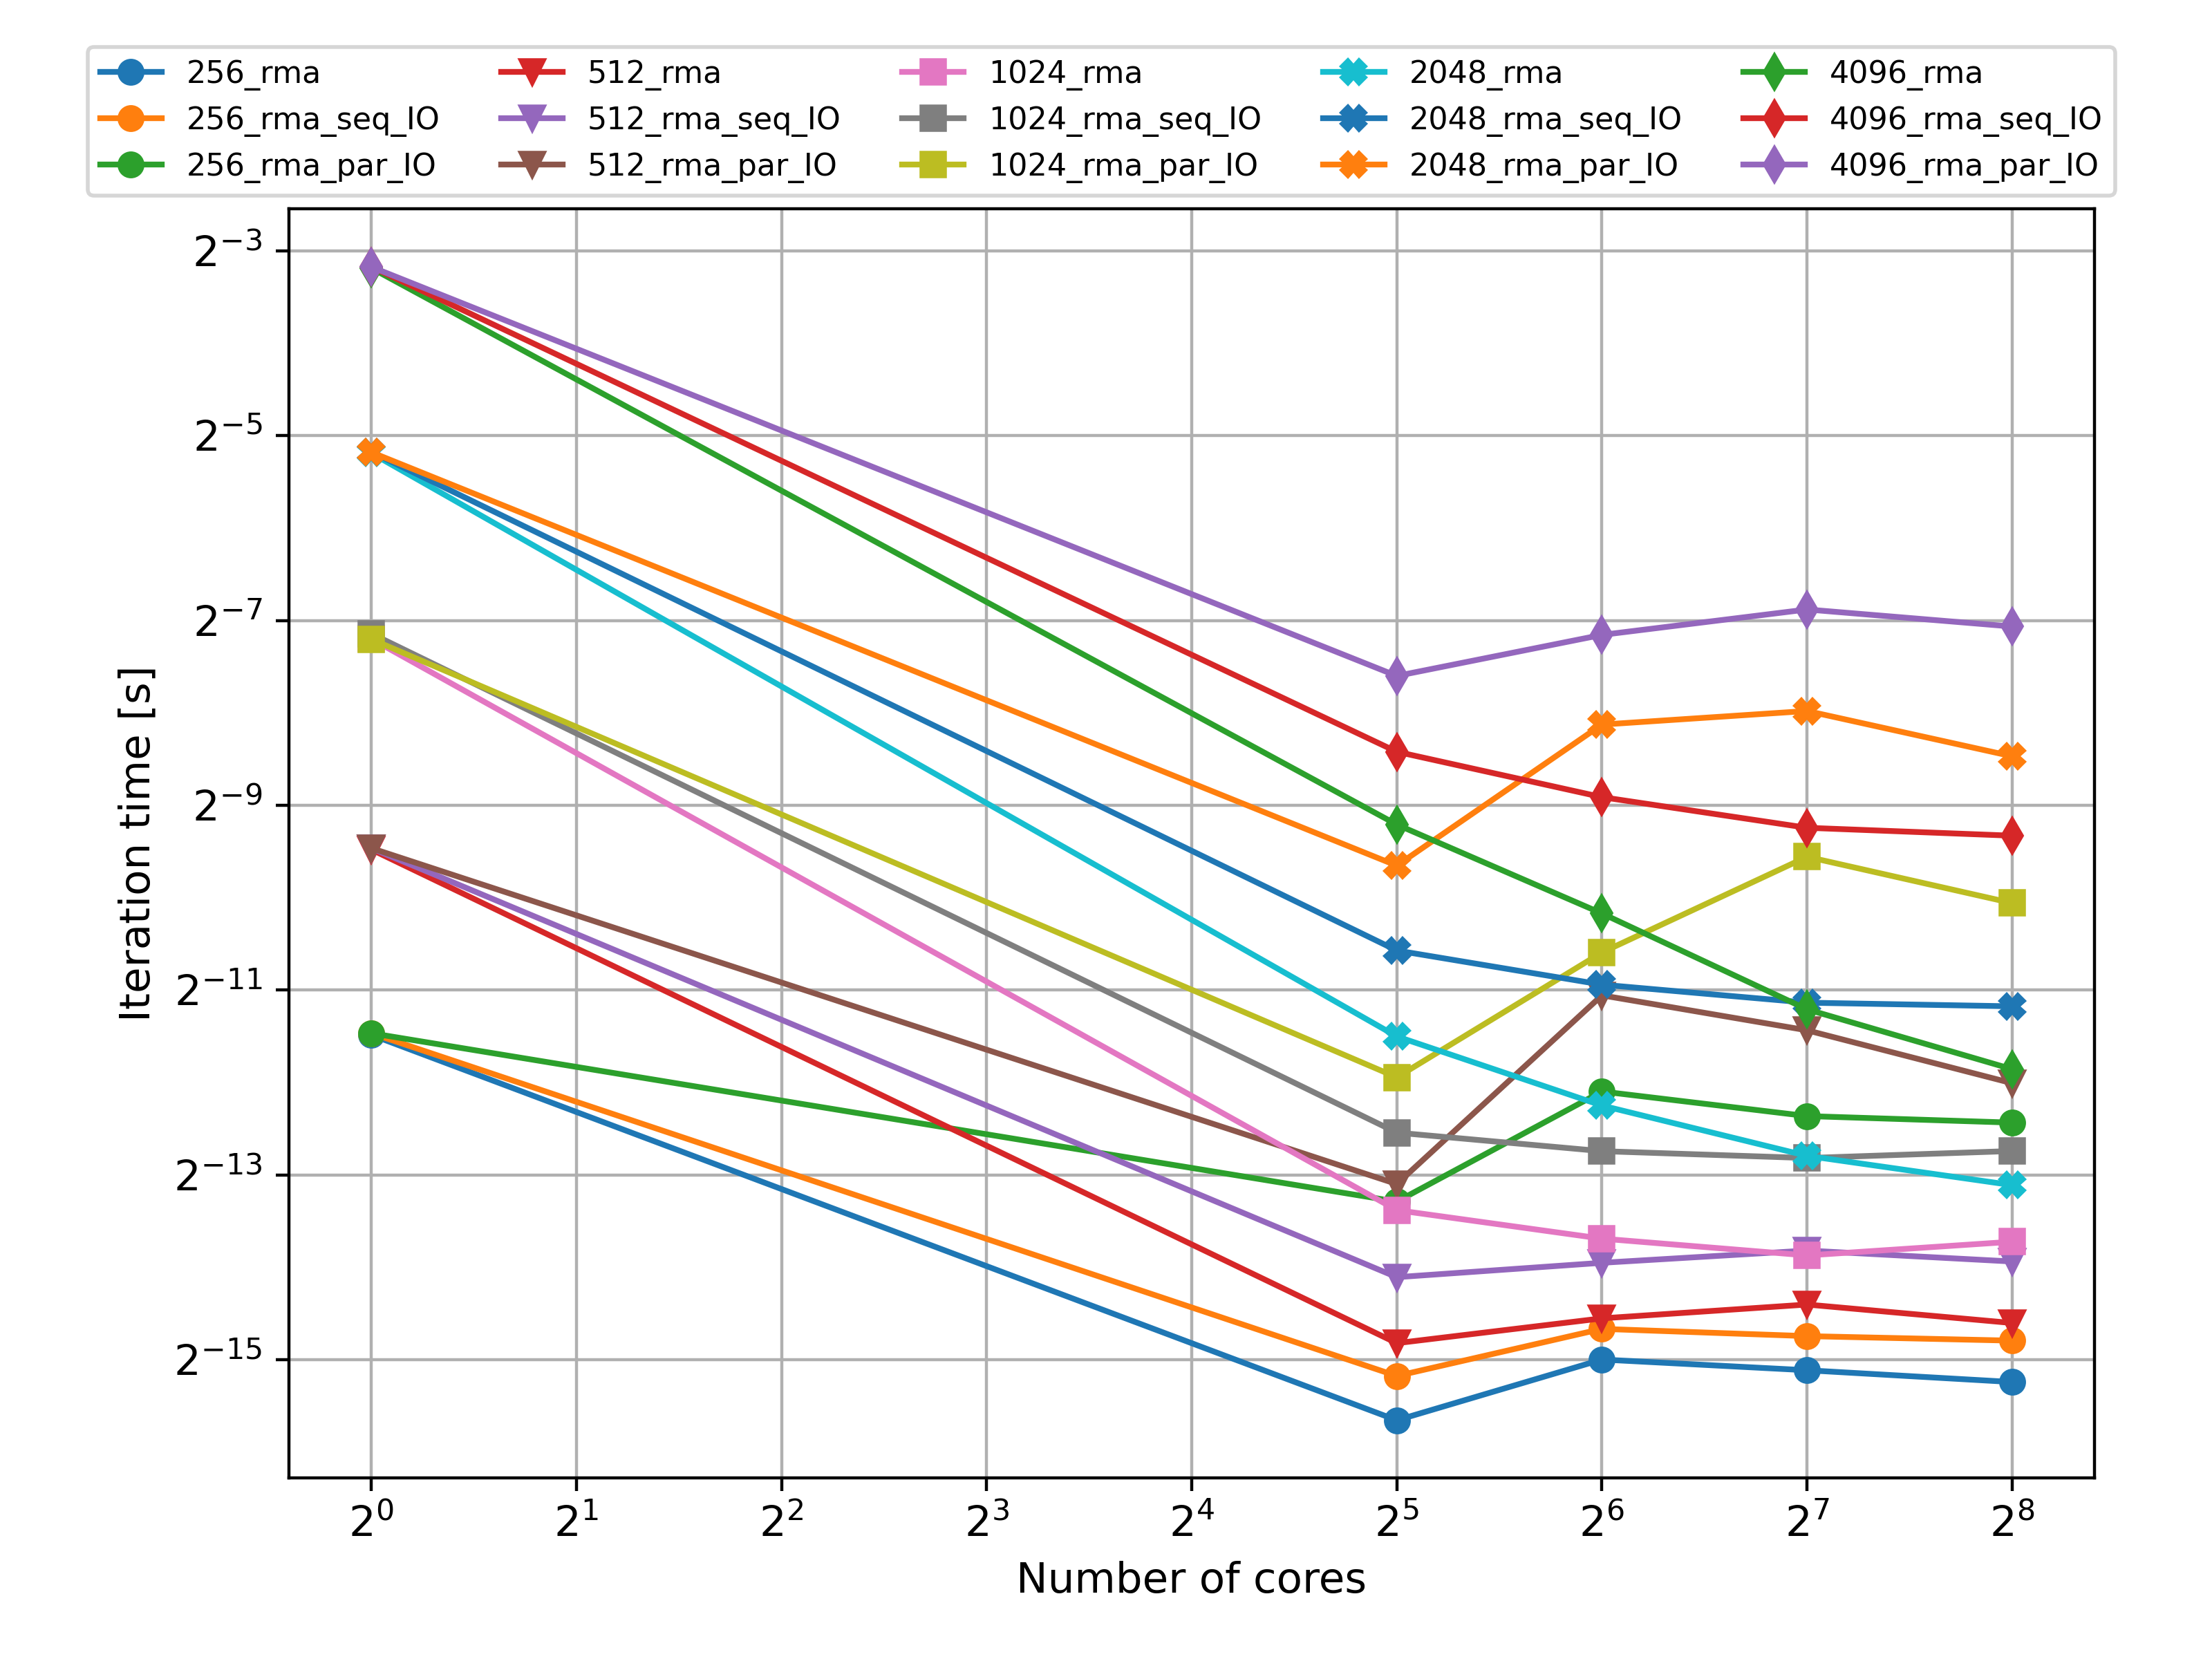
\includegraphics[width=\textwidth]{figures/ppp_scaling_hybrid_1D_rma.png}
        \caption{Cena výpočtu: hybridní MPI s 1D dekompozicí, RMA.}
        \label{fig:1D_hybrid_RMA_eff}
    \end{subfigure}
    \caption{Silné škálování a cena výpočtu: hybridní MPI s 1D dekompozicí.}
    \label{fig:1D_hybrid}
\end{figure}

% ----- Weak scaling -----
\begin{figure}[H]
    \centering
    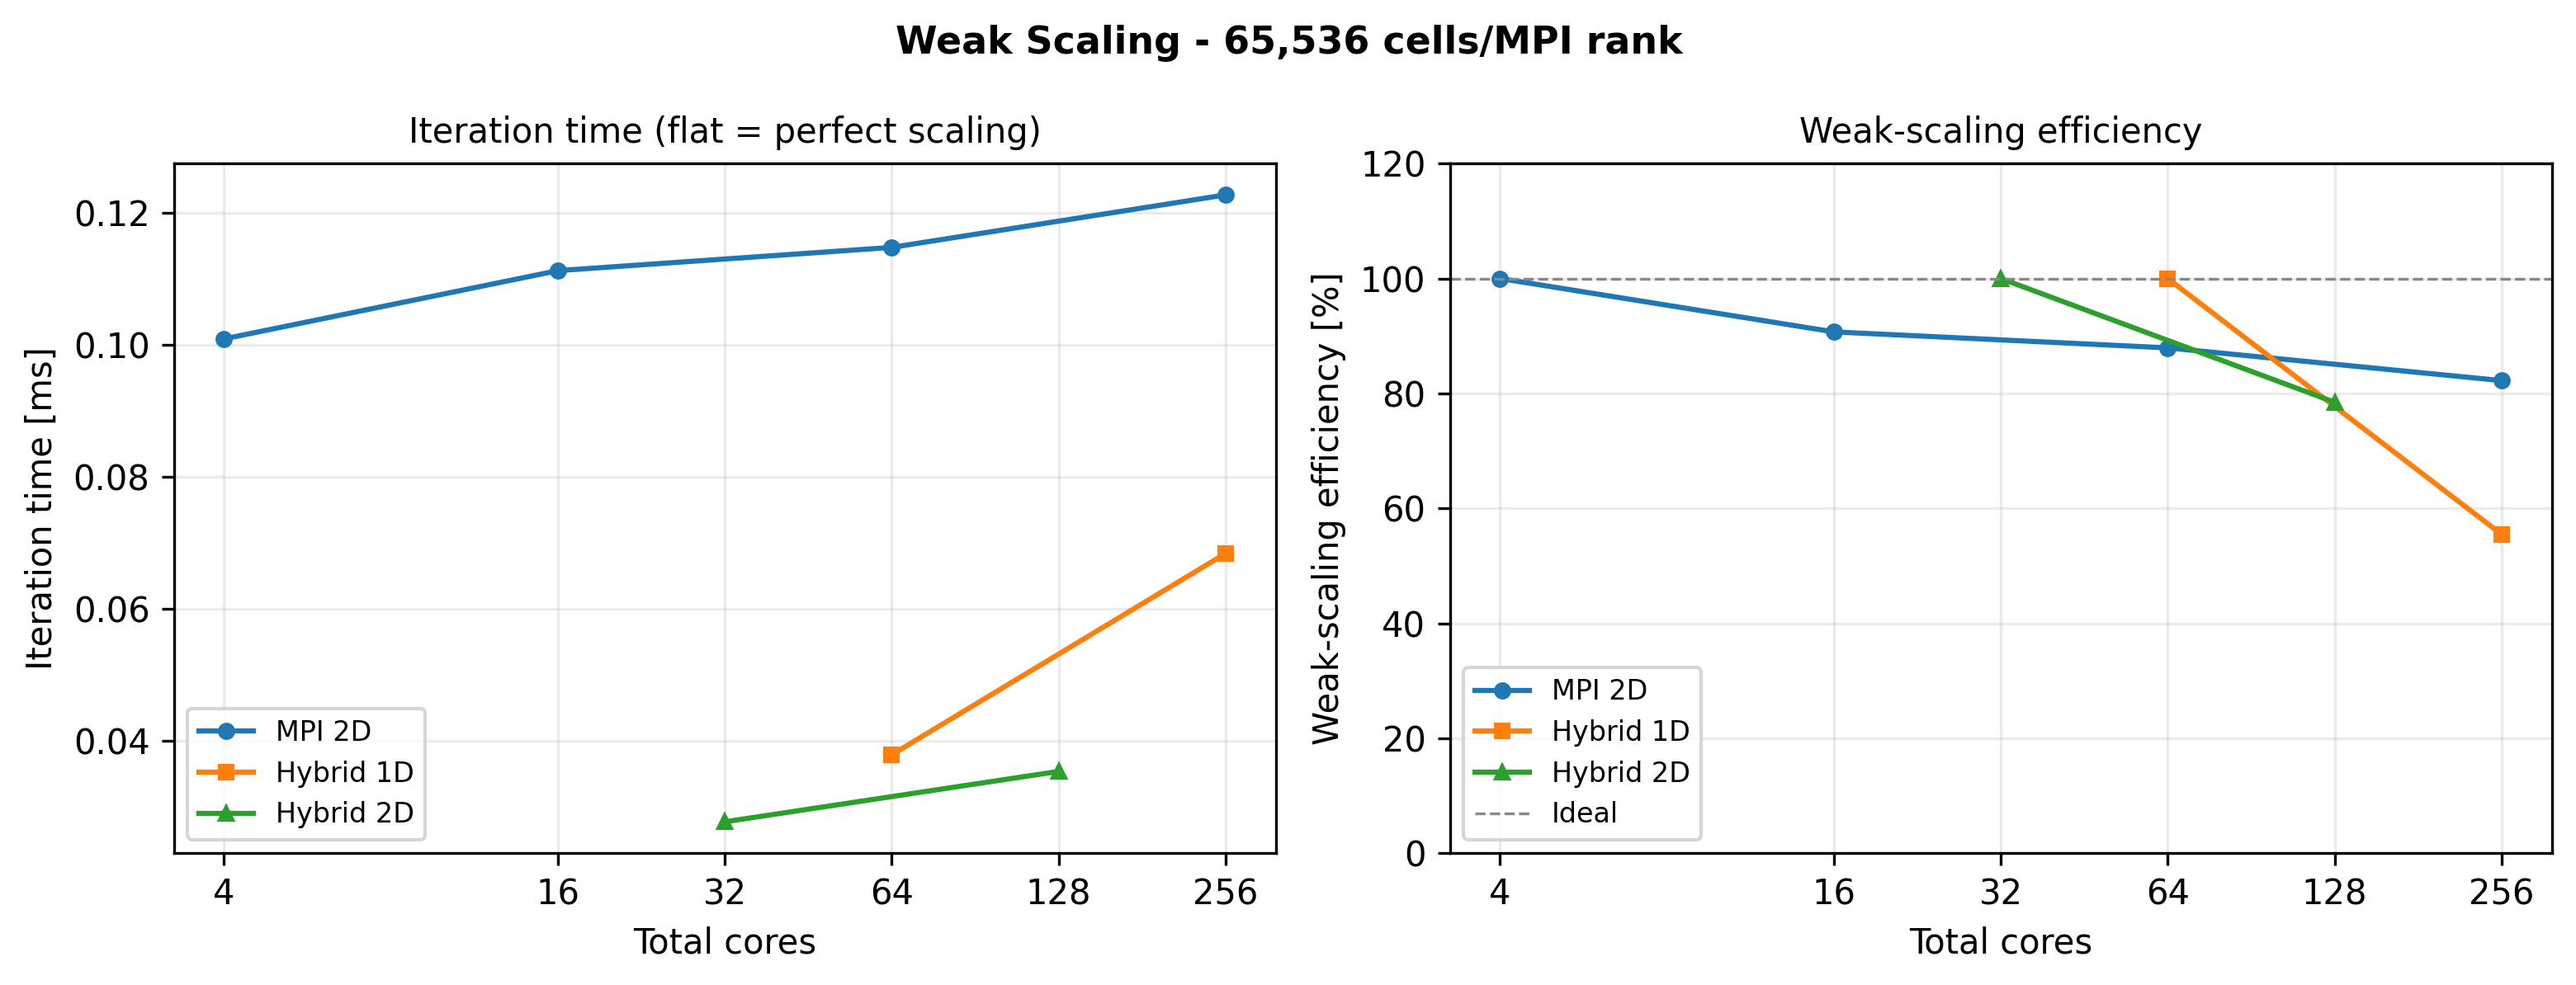
\includegraphics[width=0.6\textwidth]{figures/ppp_weak_scaling.png}
    \caption{Slabé škálování: velikost domény roste úměrně s počtem procesů
             (256$^2$/proces). Čas klesá s rostoucím $P$ díky cache efektu –
             superlineární slabé škálování.}
    \label{fig:weak_scaling}
\end{figure}

% =========================================================
\section{Profilování}
\label{sec:profilovani}
% =========================================================

% =========================================================
\subsection{Vampir}
\label{subsec:vampir}
% =========================================================

% TODO: screenshot z Vampiru po vygenerování nového Score-P profilu na Barboře
% Příkazy: rebuild build_prof, sbatch run_scorep_profile.sh

\noindent
Poznámky:
\begin{itemize}
    \item Interaktivní manuál: \url{https://vampir.eu/tutorial/manual}
    \item Process Summary: \url{https://vampir.eu/tutorial/manual/performance_data_visualization#sec-processsummary}
\end{itemize}

\begin{figure}[H]
    \centering
    \includegraphics[scale=0.5]{example-image}
    \caption{Vampir: překrytí výpočtu a komunikace, 2D dekompozice, 16 procesů, 1024$^2$.
             Zelené úseky (výpočet vnitřku dlaždice) dominují; červené MPI události
             jsou viditelné pouze na okrajích dlaždic.}
    \label{fig:vampir}
\end{figure}

% =========================================================
\subsection{Cube}
\label{subsec:cube}
% =========================================================

Starý profil (před opravami, 12. dubna) zachycuje režii \texttt{MPI\_Win\_fence}
$\approx$\,30\,\% celkového času při RMA a $\approx$\,3\,\% při P2P.
Nový profil (po PSCW a packing opravách) bude vygenerován z aktuálního
zdrojového kódu.

\begin{figure}[H]
    \centering
    \includegraphics[scale=0.5]{example-image}
    \caption{Cube: komunikační heat mapa, 2D dekompozice, 16 procesů.
             Všechny procesy odesílají stejné množství bytů – zátěž je vyrovnaná.}
    \label{fig:cube}
\end{figure}

% =========================================================
\subsection{VisIt}
\label{subsec:visit}
% =========================================================

\begin{figure}[H]
    \centering
    \includegraphics[scale=0.5]{example-image}
    \caption{VisIt: vizualizace teplotního pole, 2D doména, výsledný stav simulace.}
    \label{fig:visit}
\end{figure}

% =========================================================
\section{Závěr}
\label{sec:zaver}
% =========================================================

Implementace dosahuje superlineárního zrychlení 671$\times$ (Hybrid 2D, 256 jader,
4096$^2$) díky kombinaci cache efektu, překrytí výpočtu a komunikace,
RMA optimalizace (PSCW + packing) a opravy HDF5 chunkování.
2D dekompozice překonává 1D v 56/90 testovaných konfigurací díky
$\sqrt{P}$-krát menšímu objemu komunikace.
Paralelní I/O bylo zrychleno 4220$\times$ nastavením chunk velikosti na celou
globální doménu a konfigurací Lustre stripingu.

\end{document}
